\documentclass[a4paper]{article}
%\documentclass[doc,english]{apa}
\usepackage[utf8]{inputenc}

% packages
\usepackage{amsmath,amsfonts,amssymb, bm}
\usepackage{graphicx,verbatimbox}
\usepackage[colorlinks=true, allcolors=blue]{hyperref}
\usepackage{apacite}
\usepackage{authblk}  % for authors
\usepackage{caption}
%\usepackage{setspace} % doublespacing
\usepackage{subcaption}
\usepackage{booktabs}
\usepackage{nicefrac}
\usepackage{chngcntr} % appendix references

\usepackage{color}
\usepackage{todonotes}

%\usepackage{float}

% abbreviation Anders & Batchelder (2015)
\newcommand{\AB}{AB}

\newcommand{\EJ}[1]  {\todo[inline, color=green]{EJ: {#1}}}
\newcommand{\DON}[1] {\todo[color=orange]{Don: {#1}}}
\newcommand{\DONa}[1]{\todo[        color=white]{Don: {#1}}}


\newcommand{\Irater}{r}
\newcommand{\Iitem}{i}
\newcommand{\Ipatient}{p}
\newcommand{\Incat}{c}
\newcommand{\Ilatent}{l}

\newcommand{\Trater}{\expandafter\MakeUppercase\expandafter{\Irater}}
\newcommand{\Titem}{\expandafter\MakeUppercase\expandafter{\Iitem}}
\newcommand{\Tpatient}{\expandafter\MakeUppercase\expandafter{\Ipatient}}
\newcommand{\Tncat}{\expandafter\MakeUppercase\expandafter{\Incat}}
\newcommand{\Tlatent}{\expandafter\MakeUppercase\expandafter{\Ilatent}}

% definitions of variables
\newcommand{\ItemTruth}{\theta}
\newcommand{\ItemDifficulty}{\kappa}
\newcommand{\UnBiasedThreshold}{\gamma}
\newcommand{\Threshold}{\delta}
\newcommand{\RaterScale}{\alpha}
\newcommand{\RaterShift}{\beta}
\newcommand{\RaterCompetence}{\zeta}
\newcommand{\Appraisal}{y}
\newcommand{\Error}{\epsilon}
\newcommand{\FactorScore}{\eta}
\newcommand{\FactorRegression}{\lambda}
\newcommand{\RaterCovariate}{z}
\newcommand{\PatientCovariate}{w}


% Probability distributions

\newcommand{\ilogit}[1]{\text{logit}^{-1}\left(#1\right)}
\newcommand{\logit}[1]{\text{logit}\left(#1\right)}
\newcommand{\dnorm}[2]{\text{Normal}\left(#1,\,#2\right)}
\newcommand{\dnormp}[2]{\text{Normal\textsuperscript{+}}\left(#1,\,#2\right)}
\newcommand{\dgamma}[2]{\text{Gamma}\left(#1,\,#2\right)}
\newcommand{\dgammaMV}[2]{\text{Gamma}\left(\nicefrac{#1^2}{#2},\,\nicefrac{#1}{#2}\right)} % #1 is mean, #2 is variance
\newcommand{\dlognormal}[2]{\ensuremath{\mathrm{LogNormal}\left(#1,\,#2\right)}}
\newcommand{\dlogis}[2]{\text{Logistic}\left(#1,\,#2\right)}
\newcommand{\SE}[1]{\emph{({#1})}}

\newcommand{\code}[1]{\texttt{#1}}
%\newcommand{\dnorm}[2]{\mathcal{N}\left(#1,\,#2\right)}
%\newcommand{\dgamma}[2]{\mathcal{G}\left(#1,\,#2\right)}

\makeatletter
\renewcommand\AB@affilsepx{, \protect\Affilfont}% no newline after each affiliation
\makeatother

\newcommand{\osflink}{\url{https://osf.io/jkv38/}}

\title{Cultural Consensus Theory for the Evaluation of Patients' Mental Health Scores in Psychiatric Detention Centers}

\renewcommand{\thefootnote}{\fnsymbol{footnote}}
\author[1]{Don van den Bergh%
\thanks{Correspondence concerning this article should be addressed to: Don van den Bergh, University of Amsterdam, Department of Psychological Methods, Nieuwe Achtergracht 129, 1001 NK Amsterdam, The Netherlands. E-Mail should be sent to: donvdbergh@hotmail.com. This work was supported by a Research Talent grant from the Netherlands Organization of Scientic Research (NWO).
}}
\author[2]{Stefan Bogaerts}
\author[3]{Marinus Spreen}
\author[4]{Rob Flohr}
\author[5]{Joachim Vandekerckhove}
\author[6]{Mijke Rhemtulla}
\author[5]{William H. Batchelder}
\author[1]{Eric-Jan Wagenmakers}
\affil[1]{University of Amsterdam}
\affil[2]{University of Tilburg}
\affil[3]{Mesdag Clinic}
\affil[4]{Stenden University of Applied Sciences}
\affil[5]{University of California Irvine}
\affil[6]{University of California Davis}
\date{}
\renewcommand*{\thefootnote}{\arabic{footnote}}
\begin{document}

%\listoftodos

%\noindent Dear all,
%
%\noindent Last year, I took over Ravi Selker's project on ``A Bayesian Approach to Mental Health Assessment in Psychiatric Detention Centers''. I am writing you since you were listed in the grant proposal under collaborators. Please let me know if you are still interested in collaborating on this topic. \\
%
%\noindent Right now I am writing the a paper on cultural consensus theory which I intend to submit for the special issue in honor of William Batchelder. If you are interested, I would appreciate it if you could provide me with feedback on the current manuscript.\\
%I hope to hear from you soon.\\
%
%\noindent Kind regards,\\
%Don van den Bergh

%\newpage


\maketitle

%\vspace{-1.5em}
\begin{abstract}
In many psychiatric detention centers, patients' mental health is monitored at regular intervals. Typically, clinicians score patients using a Likert scale on multiple criteria including hostility. Having an overview of patients’ scores benefits staff members in at least three ways. First, the scores may help adjust treatment to the individual patient; second, the change in scores over time allows an assessment of treatment effectiveness; third, the scores may warn staff that particular patients are at high risk of turning violent. Practical importance notwithstanding, current practices for the analysis of mental health scores are suboptimal: evaluations from different clinicians are averaged (as if the Likert scale were linear and the clinicians identical), and patients are analyzed in isolation (as if they were independent). Uncertainty estimates of the resulting score are often ignored. Here we outline a quantitative program for the analysis of mental health scores using cultural consensus theory (CCT; \citeNP{Anders2015cultural}). CCT models take into account the ordinal nature of the Likert scale, the individual differences among clinicians, and the possible commonalities between patients. In a simulation, we compare the predictive performance of the CCT model to the current practice of aggregating raw observations and, as a more reasonable alternative, against often-used machine learning toolboxes. In addition, we outline the substantive conclusions afforded by application of the CCT model. We end with recommendations for clinical practitioners who wish to apply CCT in their work. 
\end{abstract}
\newpage

% Introduction

Psychiatric detention centers monitor the mental health of their patients at regular intervals, typically using a method such as Routine Outcome Monitoring \cite{deBeurs2011ROM}. A clinician, psychiatrist, or another staff member, henceforth a \textit{rater}, scores a patient on multiple criteria. For example, a rater evaluates a patient's behavior on a variety of criteria that relate to aggressiveness. Today, such evaluations are stored so they may be used later to inform decisions. The decisions informed by these ratings can vary widely. For instance, the scores may help adjust treatment to individual patients, the change in scores over time allows for an assessment of treatment effectiveness, and the scores may warn staff that particular patients are at high risk of turning violent. Moreover, these ratings are key for a quantitative approach to monitoring and forecasting patients' behavior.

Current practices for aggregating the scores are suboptimal. Evaluations from different raters are often averaged as if they are exchangeable. For example, personal communication with the staff of a psychiatric detention center suggested that clinicians are more lenient in their ratings than psychiatrists, but this information is not used to weigh their ratings. Furthermore, different patients are analyzed in isolation, as if they are independent. Any background information about patients, such as a patient's criminal offense, is not accounted for in a model-based manner. In addition, any uncertainty estimates of the resulting score are usually ignored.

Here, we try to address these issues using Cultural Consensus Theory \cite<CCT; >{romney1986culture, batchelder1988test, batchelder2012cultural}. The defining characteristic of CCT is that it aims to estimate the consensus knowledge shared by raters. Hence, CCT is a promising framework for analyzing data of psychiatric detention centers, where the true state of a patient is unknown and needs to be estimated from the scores given by the raters. CCT models capture individual differences between raters and items, and pool information while accounting for these differences. However, currently available CCT models can only be applied to the data of a single patient; a limitation addressed in this paper.

The focus of this paper is to outline a quantitative program for the analysis of mental health scores using CCT. First, a CCT model for ordinal data is introduced \cite{Anders2015cultural}. Afterward, this model is expanded step by step, to include more characteristics of the data, such as describing multiple patients simultaneously. We showcase the model in three simulation studies. First, we show that model parameters are retrieved accurately. Second, we demonstrate how CCT could be used to monitor patients progress over time. Third, we compare the predictive performance of the CCT model to the current practice of aggregating raw observations and, as a more reasonable alternative, against often-used machine learning toolboxes such as Random Forest \cite{breiman2001random} and Boosted Regression Trees \cite{friedman2002stochastic}. We showcase the substantive conclusions obtained from applying the CCT model and conclude the paper with recommendations for clinical practitioners who wish to apply CCT in their work.

\section*{Cultural Consensus Theory and Three Extensions}
The next sections introduce Cultural Consensus Theory (CCT). First, a brief introduction to CCT is given. Afterward, the CCT model developed in \citeA[henceforth \AB{}]{Anders2015cultural} is introduced, which serves as the simplest model for a single patient. Subsequently, we generalize the model in three ways. First, the model is expanded to describe multiple patients simultaneously. Next, latent constructs are added to the model. Finally, the model is adapted to include background information on patients and raters.

\subsection*{Cultural Consensus Theory}
Cultural Consensus Theory, also known as ``test theory without an answer key'' \cite{batchelder1988test}, is a statistical tool that attempts to retrieve the unknown ``truth'' for an item by examining the consensus among the responses. For example, given a political questionnaire, there are no objectively correct answers. Instead, one could administer the questionnaire to left-oriented respondents and use CCT to find out what the consensus is among left-oriented respondents. CCT models capture that some responders have a higher competency and will strictly answer according to the cultural consensus. Likewise, items can differ in their difficulty, i.e., the competence required to answer according to the consensus. For a political questionnaire, this implies that only extremely left-oriented respondents agree with the most left-oriented political statements. In addition, CCT models can be expanded to allow for multiple consensus truths, i.e., there can be multiple unknown truths that vary across subgroups of respondents \cite{AndersBatchelder2012}. For a political questionnaire, the different consensuses (e.g., left, right, center, etc.) and respondents membership to these groups would be estimated from the data. The property of CCT models to estimate the consensus truth from the data is ideal for psychiatric data, where a patient's true state is unknown and a consensus from the raters is desired. CCT models can be applied to continuous data \cite<e.g., the LTM;>{batchelder2012cultural}, binary data \cite<e.g.,~the General Condorcet model; >{Batchelder1986statistical}, and ordinal data (\AB{}). Since ratings are usually given on a Likert scale, we focus on a CCT model for ordinal data.

\subsection*{The Latent Truth Rater Model}
As a starting point, consider the Latent Truth Rater Model (LTRM), a cultural consensus model for ordinal data introduced by \AB{}. Figure~\ref{model:LTRM} shows a graphical model of the LTRM. The LTRM captures differences among raters and items and may be viewed as the simplest model for a single patient.
\begin{figure}[!ht]
	\begin{minipage}{0.5\textwidth}
		\centering
		\includegraphics[width=\textwidth, page=7]{graphicalModels/graphicalModels.pdf}
		\end{minipage}\hfill
	\begin{minipage}{0.5\textwidth}
		{\normalsize
		\begin{align*}
			x_{\Irater\Iitem} &\leftarrow
			\begin{cases}
			1		&\hspace{-.3cm} \text{if } \Appraisal_{\Irater\Iitem} \leq \Threshold_{\Irater 1} \\
			\Incat	&\hspace{-.3cm} \text{if } \Threshold_{\Irater, \Incat-1} < \Appraisal_{\Irater\Iitem} \leq \Threshold_{\Irater\Incat} \\
			\Tncat	&\hspace{-.3cm} \text{if } \Appraisal_{\Irater\Iitem} > \Threshold_{\Irater, \Tncat-1}
			\end{cases}\\
%			\Appraisal_{\Irater\Iitem} &\leftarrow \ItemTruth_\Iitem + \Error_{\Iitem}\\
			\Appraisal_{\Irater\Iitem} &\leftarrow \ItemTruth_\Iitem + \Error_{\Irater\Iitem}\\
			\UnBiasedThreshold_\Incat &\leftarrow \logit{\nicefrac{\Incat}{\Tncat}}\\
			\Threshold_{\Irater\Incat} &\leftarrow \RaterScale_\Irater \gamma_\Incat + \RaterShift_\Irater\\
%			\Error_{\Iitem} &\sim \dlogis{0}{\ItemDifficulty_\Iitem} \\
			\Error_{\Irater\Iitem}   &\sim \dlogis{0}{\nicefrac{\ItemDifficulty_\Iitem}{\RaterCompetence_\Irater}} \\
			\ItemTruth_\Iitem        &\sim \dnorm{\mu_\ItemTruth}{\sigma_\ItemTruth^2}\\
			\ItemDifficulty_\Iitem   &\sim \dgammaMV{\mu_\ItemDifficulty}{\sigma_\ItemDifficulty^2} \\
			\RaterScale_\Irater      &\sim \dgammaMV{\mu_{\RaterScale_\Irater}}{\sigma_{\RaterScale_\Irater}^2} \\
			\RaterShift_\Irater      &\sim \dnorm{\mu_{\RaterShift_\Irater}}{\sigma_{\RaterShift_\Irater}^2} \\
			\RaterCompetence_\Irater &\sim \dgammaMV{\mu_{\RaterCompetence_\Irater}}{\sigma_{\RaterCompetence_\Irater}^2} \\
		\end{align*}
		}%
	\end{minipage}
	\caption{Graphical model corresponding to the LTRM; a CCT model for a single patient. The hyper parameters are omitted from the graphical model. The group-level means and standard deviations are denoted $\mu$ and $\sigma$ respectively. The priors on the group-level parameters are omitted. Gamma distributions are parametrized with shape and scale so that the group-level parameters correspond to the mean and standard deviation of the distribution.}
	\label{model:LTRM}
\end{figure}
The rating of rater $\Irater$ on item $\Iitem$ is denoted $x_{\Irater\Iitem}$ and takes on discrete values from $1$ through $\Tncat$. \AB{} formalize the core ideas of the LTRM with 6 axioms, which are briefly repeated here. There is a latent, shared cultural truth among the raters, which is captured by the item location parameters $\ItemTruth_\Iitem$ (\AB{}'s axiom 1). Since raters are not perfect measurement instruments, they infer a noisy version of the cultural truth for each item, called a latent appraisal and defined as $\Appraisal_{\Iitem} = \ItemTruth_\Iitem + \Error_{\Irater\Iitem}$, where $\Error_{\Irater\Iitem}\sim \dlogis{0}{\nicefrac{\RaterCompetence_\Irater}{\ItemDifficulty_\Iitem}}$ (\AB{}'s axiom 2). 
The appraisal error $\Error_{\Irater\Iitem}$ has variance $\nicefrac{\RaterCompetence_\Irater}{\ItemDifficulty_\Iitem}$ which varies across items and raters. This reflects that items fluctuate in difficulty, captured by $\ItemDifficulty_\Iitem$ and that raters vary in competence, captured by $\RaterCompetence_\Irater$ (\AB{}'s axiom 3). Latent appraisals are assumed to be conditionally independent given the latent truth $\ItemTruth{}_\Iitem$ and the appraisal error $\Error_{\Irater\Iitem}$ (\AB{}'s axiom 4). So far, the axioms describe a continuous latent process that underlies each observation. To translate these continuous latent appraisals to categorical responses, it is assumed that there exist $\Tncat - 1$ ordered thresholds $\delta_{\Irater\Incat}$, such that each $x_{\Irater\Iitem}$ is generated deterministically in the following way (\AB{}'s axiom 5):
\begin{align*}
	x_{\Irater\Iitem} = 
	\left\{\begin{array}{ll} 
	1		& \text{if }  \Appraisal_{\Irater\Iitem} \leq \Threshold_{\Irater 1} \\[4pt]
	\Incat	& \text{if }  \Threshold_{\Irater, \Incat-1} <  \Appraisal_{\Irater\Iitem} \leq \Threshold_{\Irater\Incat} \\[4pt]
	\Tncat	& \text{if }  \Appraisal_{\Irater\Iitem} > \Threshold_{\Irater, \Tncat-1}
	\end{array} \right.
\end{align*}
The appraisal $\Appraisal_{\Irater\Iitem}$ is latent and thus we consider the probability that an appraisal fails in between two thresholds to obtain the probability of an observed score. This makes the generating process of $x_{\Irater\Iitem}$ probabilistic and described by an ordered logistic distribution\footnote{The choice for an ordered logistic distribution is arbitrary and an ordered probit distribution could also be used, as was done by \AB{}.}, which gives:
\begin{align*}
P(x_{\Irater\Iitem}\mid  \Appraisal_{\Irater\Iitem},\delta_{\Irater}) = 
\left\{\begin{array}{ll} 
1 - \ilogit{\Appraisal_{\Irater\Iitem} - \Threshold_{\Irater 1}}         & \text{if } x_{\Irater\Iitem} = 1, \\[4pt]
	\ilogit{\Appraisal_{\Irater\Iitem} - \Threshold_{\Irater,\Incat-1}} - 
	\ilogit{\Appraisal_{\Irater\Iitem} - \Threshold_{\Irater\Incat}}         & \text{if } 1 < x_{\Irater\Iitem} < \Tncat,\\[4pt]
	\ilogit{\Appraisal_{\Irater\Iitem} - \Threshold_{\Irater,\Tncat-1}}       & \text{if } x_{\Irater\Iitem} = \Tncat. 
\end{array} \right.
\end{align*}
The thresholds $\Threshold_{\Irater\Incat}$ accommodate the response biases of the raters. \AB{} do so by estimating $\Tncat-1$ ordered thresholds $\UnBiasedThreshold$ and defining $\Threshold_{\Irater\Incat} = \RaterScale_\Irater \UnBiasedThreshold_\Incat + \RaterShift_\Irater$ (\AB{}'s axiom 6). This translation of thresholds is called the Linear in Log Odds function and is a useful tool for capturing bias in probability estimation \cite{Fox1995, Gonzalez1999, Anders2015cultural}.

Figure~\ref{fig:orderedLogistic} provides an intuition for how the ordered logistic distribution can model different outcomes by varying only the rater parameters. The latent appraisal $\Appraisal$ is fixed to 0, the thresholds $\UnBiasedThreshold$ are equal to $\logit{c/C}$ such that $P(x_{\Irater\Iitem}\mid \Appraisal=0,\,\UnBiasedThreshold,\,\RaterScale_\Irater=1,\,\RaterShift_\Irater=0)$ is uniform, and the scale $\RaterScale_\Irater$ and shift $\RaterShift_\Irater$ vary. In the left panel, there is no response bias, $\RaterScale_\Irater = 1$ and $\RaterShift_\Irater = 0$, which yields a uniform distribution over the predicted Likert scores. In the right panel, an increase in response scale and shift, $\RaterShift_\Irater = .5$ and $\RaterScale_\Irater = 2$, concentrates the predicted Likert scores around 2 and 3.
\begin{figure}[!ht]
	\centering
	\begin{subfigure}{.5\textwidth}
		\centering
		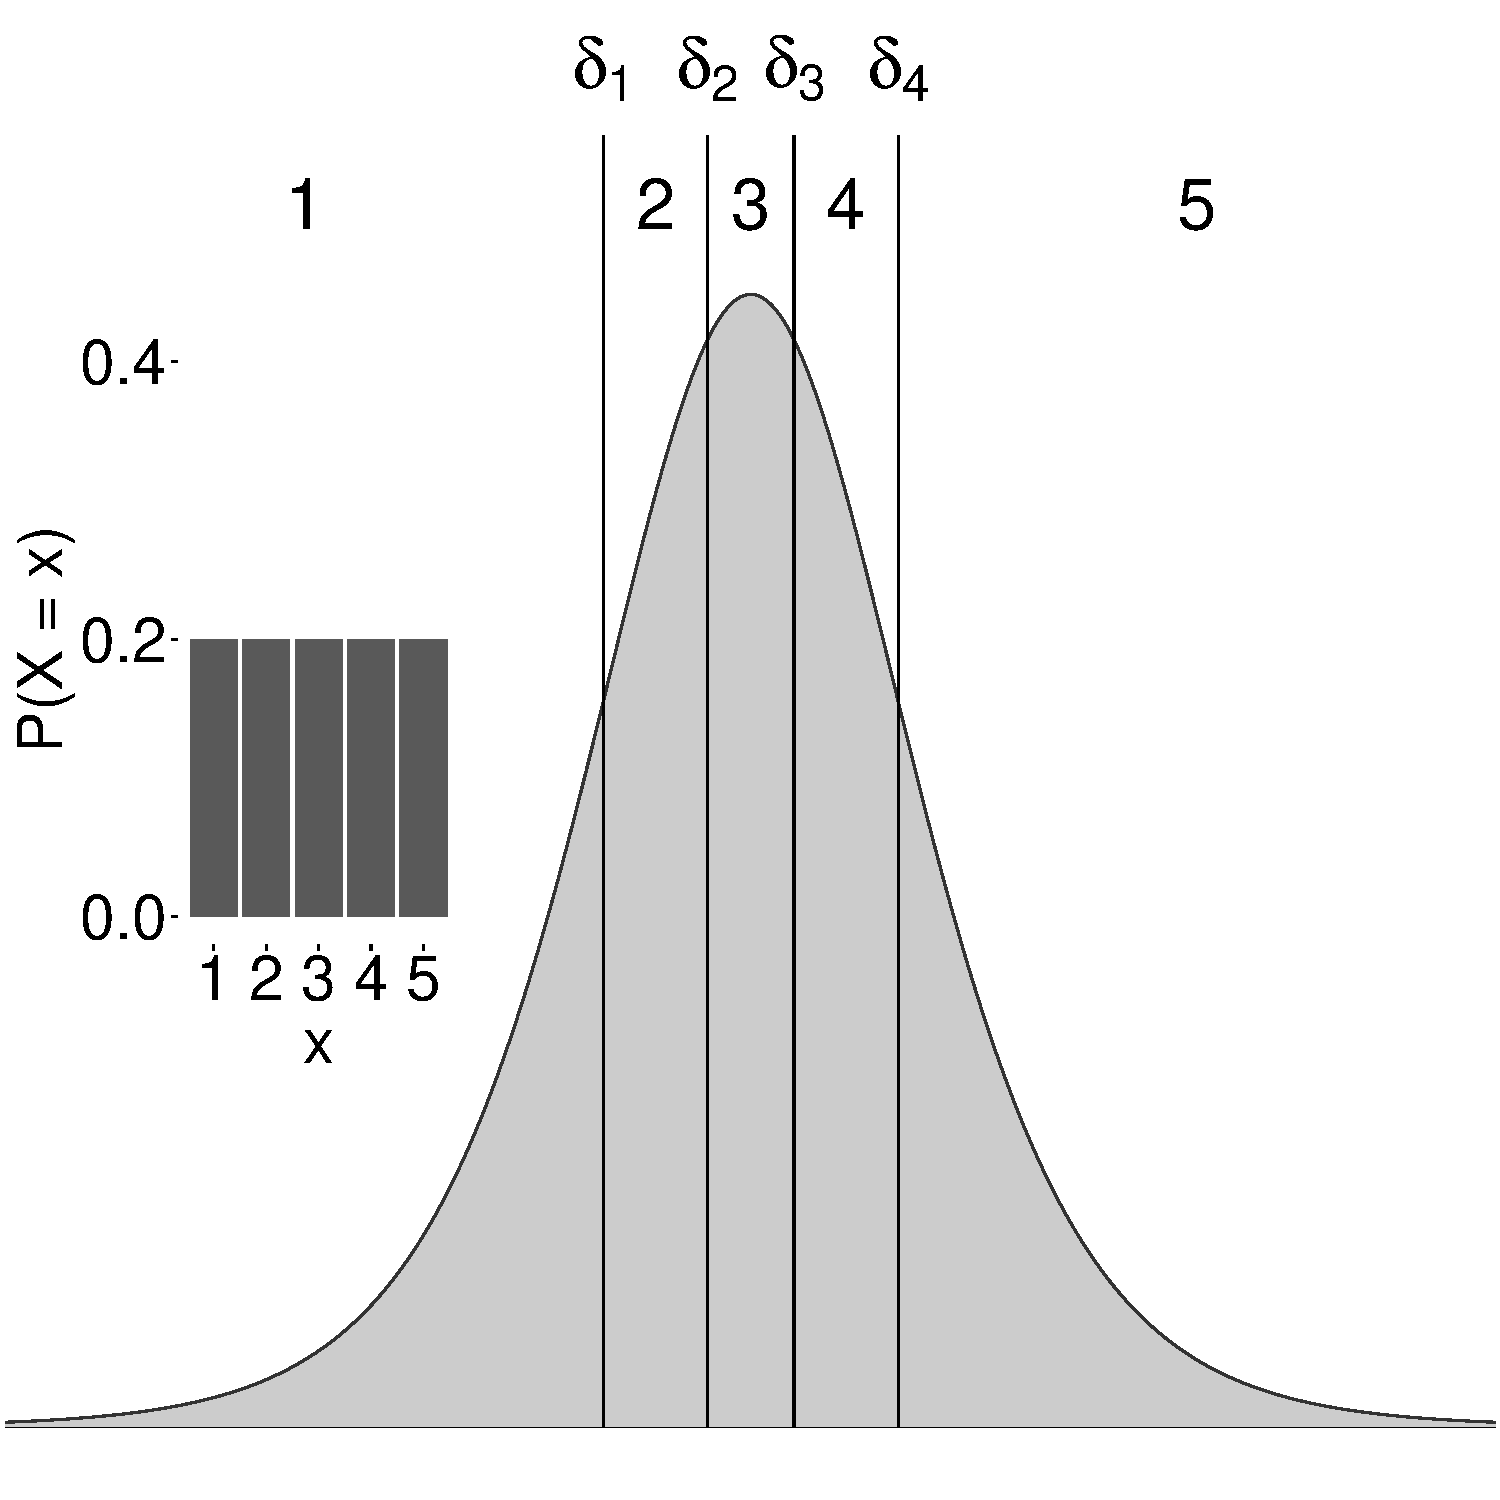
\includegraphics[width=.97\textwidth]{figures/orderedLogisticUnbiased.pdf}
	\end{subfigure}%
	\begin{subfigure}{.5\textwidth}
		\centering
		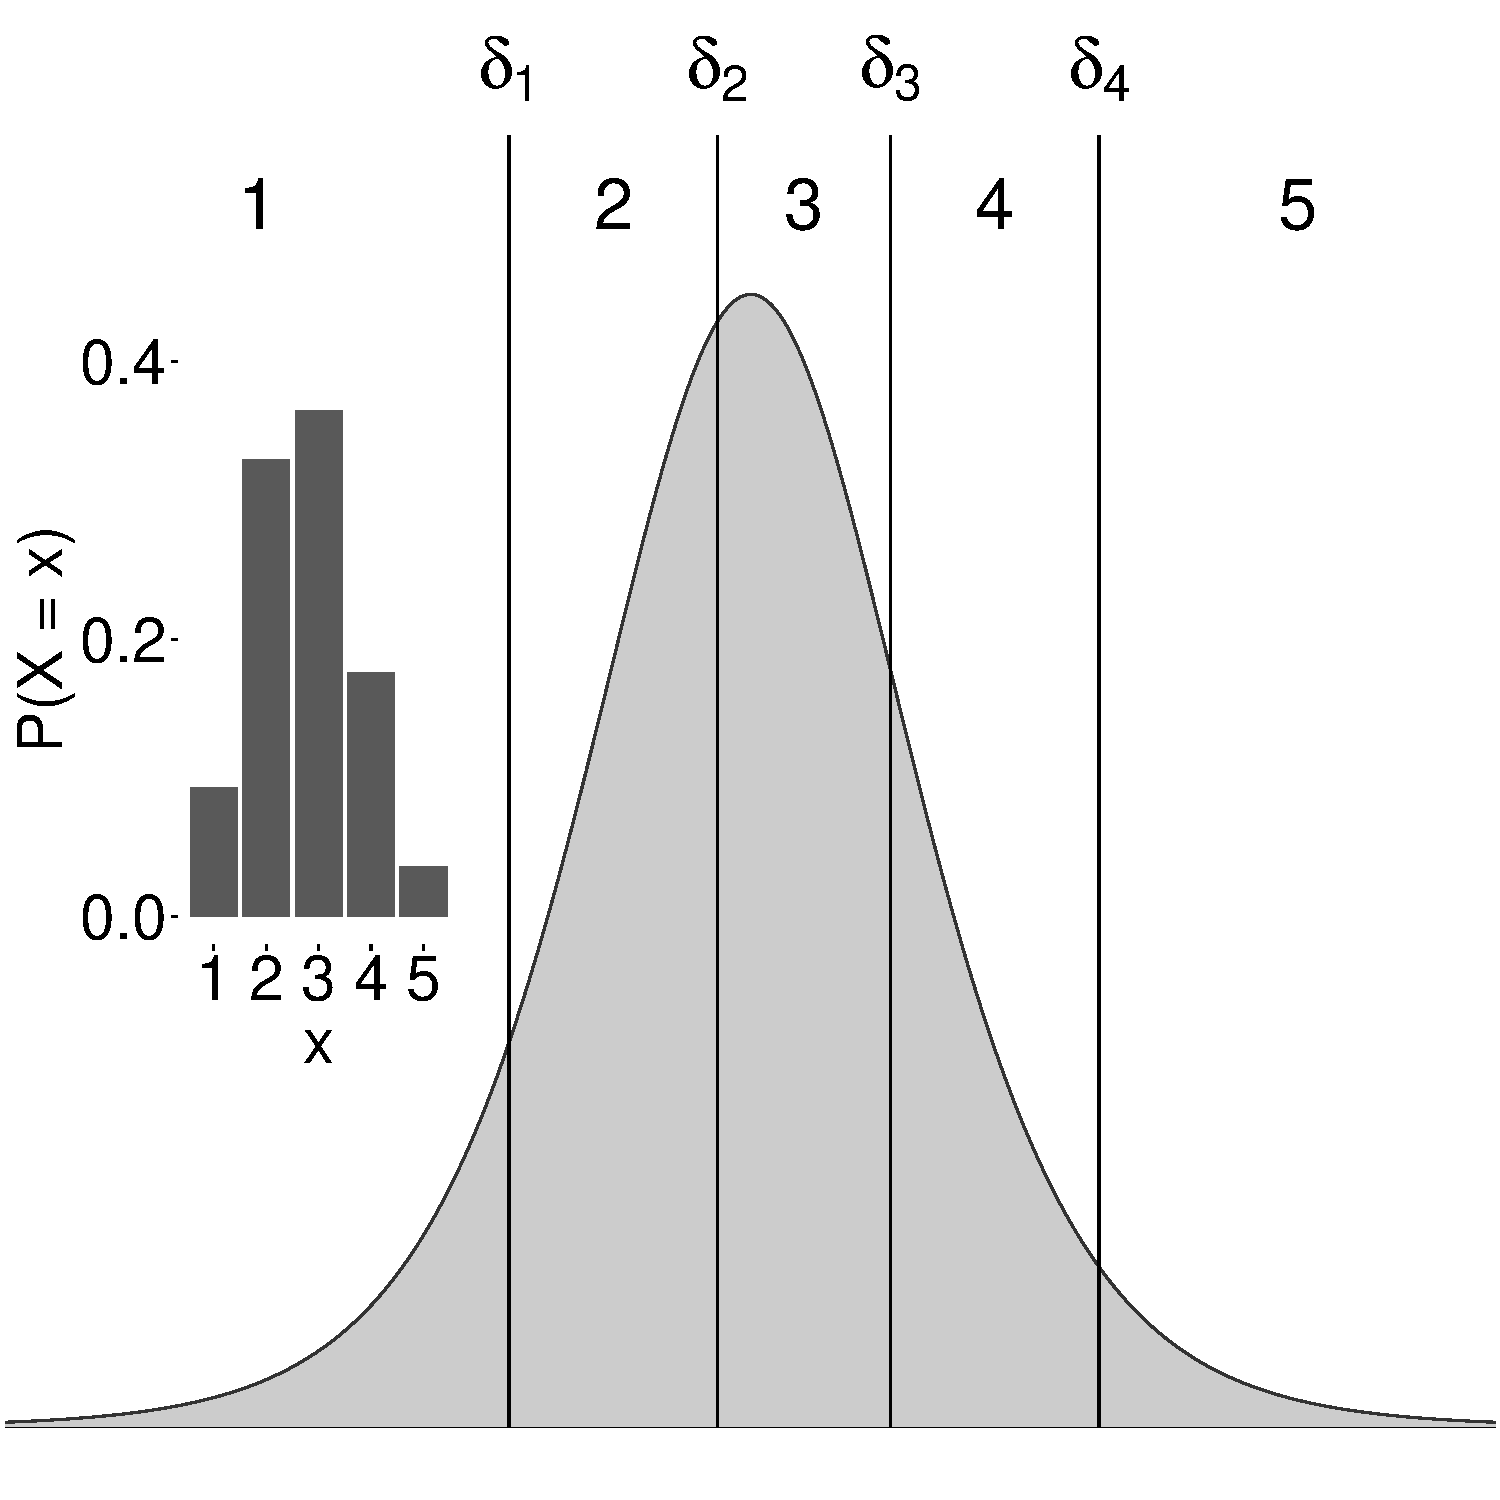
\includegraphics[width=.97\textwidth]{figures/orderedLogisticBiased.pdf}
	\end{subfigure}
	\caption{Ordered logistic distribution for $y_{\Irater\Iitem} = 0$, thresholds $\UnBiasedThreshold$ equal to $\logit{c/C}$, and varying rater components. The implied probability distribution over response categories is shown inside each panel. In the left panel, there is no response bias, $\RaterScale_\Irater = 1$, $\RaterShift_\Irater = 0$. As a consequence, the distribution over the predicted Likert scores is uniform. In the right panel, the thresholds are shifted right, $\RaterShift_\Irater = 0.5$, and the scale increased slightly, $\RaterScale_\Irater = 2$, such that the distribution over predicted Likert scores is peaked on outcomes 2 and 3.}
	\label{fig:orderedLogistic}
\end{figure}

The LTRM is a complex model and unfortunately suffers from identification issues, as was pointed out by \AB{} already. For example, multiplying the rater competences $\RaterCompetence$ and the item difficulties $\ItemDifficulty$ by a constant $c$ yields an identical variance for the appraisal distribution since $\nicefrac{c\RaterCompetence}{c\ItemDifficulty} = \nicefrac{\RaterCompetence}{\ItemDifficulty}$. Such identification problems are avoided by restricting the mean of the respective parameters to 1 (as suggested in Appendix C in \AB{}).
Another identification problem originates from estimating the thresholds individually. The number of thresholds, $\Tncat-1$, increases with the number of response options. This introduces a large number of parameters that can be difficult to estimate, in particular when some response options are not observed (i.e., when there are ceiling or floor effects). In addition, the model is only identified if the sum of thresholds is zero ($\sum_{\Incat=1}^{\Tncat}\UnBiasedThreshold_\Incat = 0$; otherwise adding a constant to $\ItemTruth{}_\Iitem$ and $\Threshold_\Incat$ yields an identical likelihood). Rather than modeling each threshold individually, we describe the thresholds using only two parameters per rater. Specifically, we model the thresholds as deviances from an initial guess, $\UnBiasedThreshold_\Incat = \logit{c/C}$. This yields a set of thresholds such that if the latent appraisal is 0 then $P(x_{\Irater\Iitem})$ is uniform. Response biases are incorporated in the same manner: $\Threshold_{\Irater\Incat} = \RaterScale_\Irater\logit{c/C} + \RaterShift_\Irater$. This simplification can still capture a wide variety of data sets \cite{Selker2019}. 

\subsection*{Three Extensions}

The LTRM as described above has many desired properties, for instance, it captures individual differences among both raters and items. However, many properties of psychiatric data are not captured by the model. three sections generalize the LTRM to improve its capacity to describe the data at hand.

\subsubsection*{Extension I: Multiple Patients}
The first extension allows the model to describe multiple patients. Since different patients can have different mental disorders the latent truth for an item varies across patients to reflect this. Likewise, some items may be more difficult to measure, but only for some patients. Both these changes can be achieved by allowing the item truth $\ItemTruth_{\Iitem\Ipatient}$ and item difficulty $\ItemDifficulty_{\Iitem\Ipatient}$ to vary across patients. In turn, this induces that the latent appraisal $\Appraisal_{\Irater\Iitem\Ipatient}$ varies across patients. As in Figure~\ref{model:LTRM}, we assume that the patient parameters are drawn from a group-level distribution with unknown mean and variance, for instance, the item difficulty could follow a gamma distribution with unknown mean and variance (i.e., $\ItemDifficulty_{\Iitem\Ipatient} \sim \dgammaMV{\mu_\ItemDifficulty}{\sigma_\ItemDifficulty^2}$).

\subsubsection*{Extension II: Latent Constructs}
Often, we are not just interested in the latent truth of a single item, but also in a construct that is measured by multiple items. For instance, the latent construct aggressiveness could be measured with multiple items. To accomplish this, we introduce a latent variable $\FactorScore_{\Ipatient\Ilatent}$ and allow items to load on this latent variable, i.e., we introduce a factor model over the items. The relation between the latent construct and the item consensuses is given by the regression weights $\FactorRegression_{\Iitem\Ilatent}$, such that $\ItemTruth_{\Iitem\Ipatient} \sim \dnorm{\FactorRegression_{\Iitem\Ilatent}\eta_{\Ilatent\Ipatient}}{\sigma^2_{\FactorScore_{\Ipatient}}}$. The measurement model, i.e., which items load on what construct, is assumed to be known.

As prior distribution on the latent constructs $\FactorScore_{\Ilatent\Ipatient}$ we used a normal distribution with variance 1, which reflects that the variance of a latent variable is unidentified and restricted to 1. In addition, simulations showed that the estimated regressions weights and the estimated patients' scores on the latent constructs exhibited label switching. For example, multiplying both the latent constructs $\FactorScore$ and the regression weights $\FactorRegression$ by $-1$ yields the same distribution over the item truths. To avoid label switching, we restricted the regression weights to be positive, motivated from the perspective that it is typically known which items are negatively scored (i.e., have a negative correlation with the latent construct).

\subsubsection*{Extension III: Patient and Rater Information}
The third extension adds background information about raters and patients to the LTRM. This helps the model to capture that, for instance, pedophiles are typically less aggressive than murderers. Discrete patient and raters characteristics are captured by dividing the group-level distributions into separate components for each category. For example, the hierarchical distribution over latent variables becomes $\FactorScore_{\Ipatient\Ilatent} \sim \dnorm{\mu_{\mathrm{Crime}_\Ipatient}}{\sigma_{\mathrm{Crime}_\Ipatient}}$, where the mean and variance of the latent construct vary across patients that committed different crimes. Rater characteristics are incorporated similarly, except that these would influence the group-level distributions of rater-specific parameters. This yields $\RaterShift_\Irater \sim \dnorm{\mu_{\mathrm{Staff}_\Irater}}{\sigma_{\mathrm{Staff}_\Irater}}$. For instance, this could capture that particular groups of staff members may give more lenient ratings.

In the simulation studies, we restrict the analysis to discrete background information. However, continuous background information could also be used. Consider for instance the time a patient is committed to a detention center, $\mathrm{Time}_\Ipatient$.  This information can be added as a regression on the mean of the group-level distribution. Thus, $\FactorScore_{\Ipatient\Ilatent} \sim \dnorm{\mu_{\mathrm{Crime}_\Ipatient} + \nu\,\mathrm{Time}_\Ipatient}{\sigma_{\mathrm{Crime}_\Ipatient}}$, where $\nu$ is the regression coefficient from the time a patient is committed $\mathrm{Time}_\Ipatient$ on the mean of the group-level distribution.

It is important to consider that the influence of background variables can differ across latent constructs. For instance, the effect of a patient's crime varies across latent constructs, allowing the model to capture that pedophiles and murderers differ in aggression, but not on depression. This is accomplished by estimating the effect of a patient's crime separately for each latent construct, which implies $\mu_{\Ilatent, \mathrm{Crime}_\Ipatient}$.

\begin{figure}[!ht]
	%	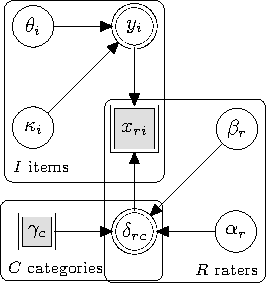
\includegraphics[width=.4\textwidth, page=1]{graphicalModels/graphicalModels.pdf}
	\begin{minipage}{0.6\textwidth}
		\centering
		\includegraphics[width=1\textwidth, page=8]{graphicalModels/graphicalModels.pdf}
	\end{minipage}\hfill
\begin{minipage}{0.4\textwidth}
{\large
	\begin{align*}
%	x_{\Irater\Iitem} &\leftarrow 
%	\begin{cases}
%	1		&\hspace{-.3cm} \text{if }  \Appraisal{}_{\Irater\Iitem} \leq \delta_{\Irater 1} \\
%	\Incat	&\hspace{-.3cm} \text{if } \delta_{\Irater, \Incat-1} <  \Appraisal{}_{\Irater\Iitem} \leq \delta_{\Irater\Incat} \\
%	\Tncat	&\hspace{-.3cm} \text{if }  \Appraisal{}_{\Irater\Iitem} > \delta_{\Irater, \Tncat-1}
%	\end{cases}\\
%	y_{\Irater\Iitem} &\leftarrow T_\Iitem + \Error_{\Irater\Iitem}\\
%	\gamma_\Incat &\leftarrow \logit{\Incat / \Tncat}\\
%	\delta_{\Irater\Incat} &\leftarrow a_\Irater  \gamma_\Incat + b_\Irater\\
%	\sigma^\Error_{\Irater\Iitem} &\leftarrow \ItemDifficulty_\Irater / \zeta_\Irater\\
%	\Error_{\Irater\Iitem} &\sim \dnorm{0}{\sigma^\Error_{\Irater\Iitem}} \\
	\ItemTruth_{\Iitem\Ipatient} &\sim \dnorm{\lambda_{\Iitem\Ilatent}\eta_{\Ilatent\Ipatient}}{1}\\
	\FactorScore_{\Ilatent\Ipatient} &\sim \dnorm{\PatientCovariate_{\Ilatent\Ipatient}}{10} \\
%	\FactorRegression_{\Iitem\Ilatent} &\sim \dgamma{0.01}{0.01} \\
	\FactorRegression_{\Iitem\Ilatent} &\sim \dnormp{0}{10} \\
	\RaterShift_\Irater   &\sim \dnorm{\RaterCovariate_\Irater}{\sigma_{\RaterShift_\Irater}^2}\\
	\PatientCovariate_{\Ipatient\Ilatent} & \sim\dnorm{0}{10} \\
	\RaterCovariate_\Irater &\sim \dnorm{0}{10}
%	\ItemDifficulty_\Iitem &\sim \dgammaMV{\mu_\ItemDifficulty}{\sigma_\ItemDifficulty^2} \\
%	\RaterScale_\Irater    &\sim \dgammaMV{\mu_{\RaterScale_\Irater}}{\sigma_{\RaterScale_\Irater}^2} \\
%	\RaterShift_\Irater    &\sim \dnorm{\mu_{\RaterShift_\Irater}}{\sigma_{\RaterShift_\Irater}^2}
	\end{align*}
}%
\end{minipage}
	\caption{Graphical model corresponding to the CCT model for multiple patients. Rater characteristics are captured by $\RaterCovariate_\Irater$ and patient characteristics are captured by $\PatientCovariate_{\Ilatent\Ipatient}$. The prior distributions for the extended LTRM were chosen to be uninformative.}% (for positive parameters a $\dgamma{0.01}{0.01}$ was used and a $\dnorm{0}{10}$ otherwise).}
	\label{model:LTRM3}
\end{figure}

%The prior distributions for the extended LTRM were chosen to be uninformative. The prior distribution on the latent constructs $\FactorScore_{\Ilatent\Ipatient}$ reflects that the variance of a latent variable is unidentified and restricted to 1. In simulations we noticed that the regressions from the latent construct exhibited label switching (e.g., multiplying both the latent constructs and the regression weights by $-1$ yields the same prior on the item truths). To avoid this, we restricted the regression weights to be positive. 

Figure~\ref{model:LTRM3} graphically summarizes the extended LTRM. The extended LTRM first separates the rater-specific influences from the data $x_{\Irater\Iitem\Ipatient}$, hereby accounting for different groups of raters. This results in a latent consensus for each item and patient $\ItemTruth_{\Iitem\Ipatient}$. This consensus is subsequently used as an indicator for a latent construct for all patients and constructs $\FactorScore_{\Ipatient\Ilatent}$. The relation between the latent construct and the items is given by the regression weights $\FactorRegression_{\Iitem\Ilatent}$, such that $\ItemTruth_{\Iitem\Ipatient} \sim \dnorm{\FactorRegression_{\Iitem\Ilatent}\eta_{\Ilatent\Ipatient}}{1}$. The factor scores also incorporate patient-specific background information, such as the crime a patient committed.

\section*{Implementation}
The next sections illustrate the LTRM in a variety of scenarios. First, we demonstrate the benefit of the LTRM over the raw means in an example analysis of two fictitious patients. Second, we demonstrate that the parameters of the LTRM can be accurately recovered. Last, we compare the predictive performance of the LTRM to the unweighted mean of the observations and two machine learning toolboxes.

We estimate the parameters of the LTRM and the extended LTRM using a Bayesian approach. Therefore, we are interested in the posterior distributions of the model parameters. All models were written in Stan and approximated the posterior distributions with variational inference \cite{CarpenterEtAl2017Stan}. We opted to use variational inference over traditional Markov chain Monte Carlo because it was computationally fast while providing similar results in terms of parameter retrieval and model predictions. All data was simulated using R \cite{R} and Stan models were run using the R package \code{RStan} \cite{rstan2019a2192}. R files and Stan models are available in the online appendix at \osflink{}.

\section*{Example Analysis}

Here we showcase the benefits of a CCT analysis by examining results for two fictitious participants. This example demonstrates how misleading the sample mean can be. We simulated a data set of 50 patients, 10 raters, 20 items, and 5 answer categories. The items loaded on 3 different latent constructs, further referred to as aggressiveness, anxiety, and depression. A patient-specific covariate consisting of 5 categories was added to mimic the effect of a patient's criminal offense. Similarly, two different categories were used to imitate the different groups of raters (e.g., clinicians and psychiatrists). Next, we selected two patients whose differences in observed means were small relative to their differences in posterior means on the latent constructs. The overall mean of the observed ratings was 3.51 and 3.08 for patient 1 and 2 respectively. The means for items of each construct are shown in Table~\ref{tb:rawMeans}.
\begin{table}[!ht]
	\centering
	\caption{Raw means of the observed ratings for the two patients with similar mean responses. The standard errors of the means are shown in brackets. The means and standard errors are computed for each latent construct.}% and for all scores (overall).}
	\label{tb:rawMeans}
	\begin{tabular}{rrrr}
		\toprule
		\multicolumn{1}{c}{} & \multicolumn{3}{c}{Construct}\\% & \\
		\cmidrule[0.4pt]{2-4}
		& Aggressiveness & Anxiety & Depression\\%  & Overall \\ 
		\midrule
		Patient 1 & 3.86 \SE{0.14} & 3.04 \SE{0.19} & 3.65 \SE{0.18} \\% & 3.51 \\ 
		Patient 2 & 3.29 \SE{0.17} & 3.00 \SE{0.18} & 2.93 \SE{0.21} \\% & 3.08 \\ 
		\bottomrule
	\end{tabular}
\end{table}
Analyzing these patients independently by aggregating the raw observations indicates that these two patients might differ in aggressiveness and depression but not in anxiety. However, after fitting the extended LTRM to the data it becomes apparent that there is more to the data than what is shown by these averages. Using the extended LTRM, we can visualize the posterior distributions of the latent constructs for both patients, shown in Figure~\ref{fig:ExamplePosterior}.
\begin{figure}[!ht]
	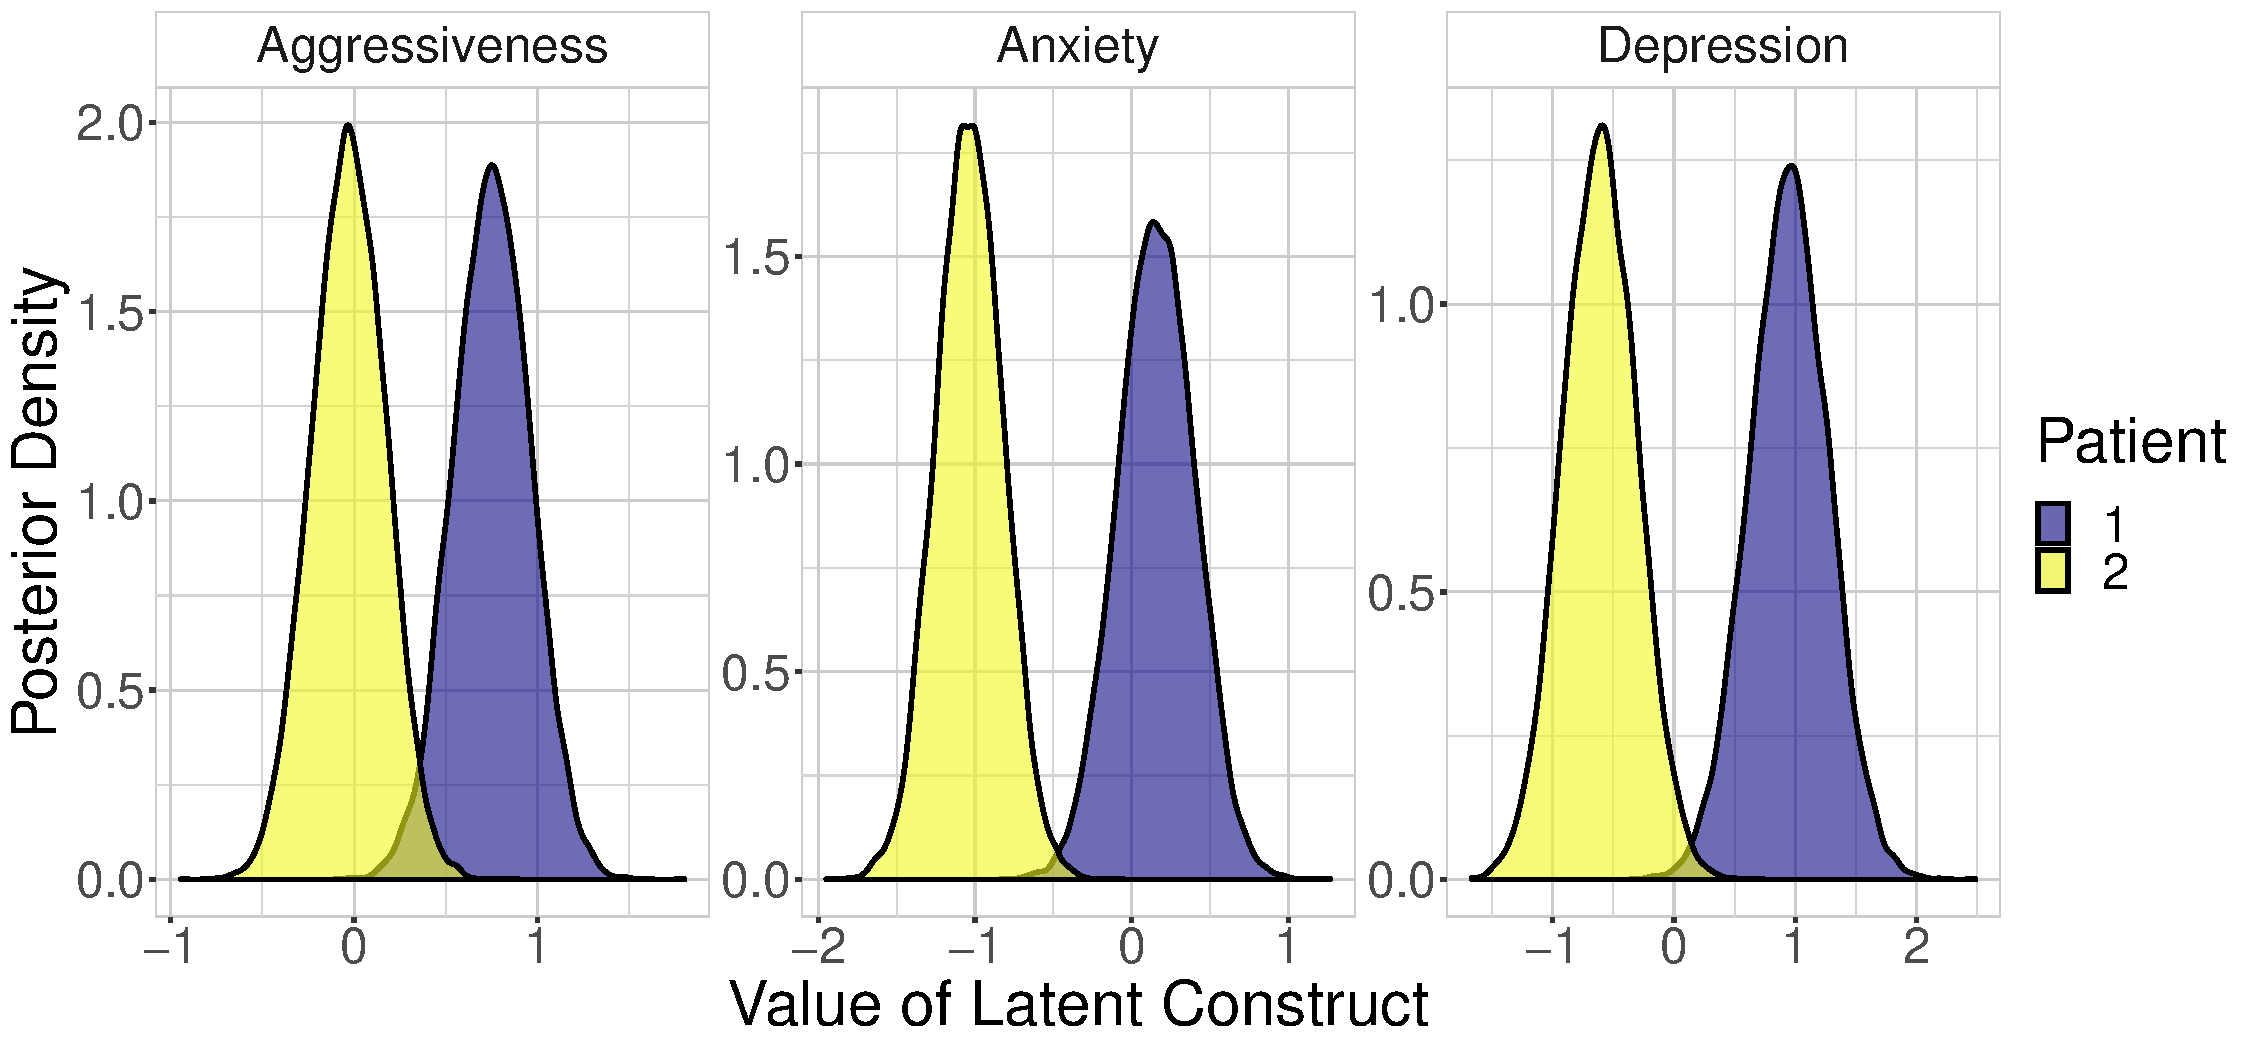
\includegraphics[width=\textwidth]{figures/twoPatientsDensity.pdf}
	\caption{Approximate posterior densities for the two patients similar response pattern. The panels show different latent constructs. The posterior distributions suggest these patients differ on all three latent constructs, unlike what the raw means in Table~\ref{tb:rawMeans} would suggest. This demonstrates that more information can be obtained from the ratings than what may be obvious from the raw scores.}
	\label{fig:ExamplePosterior}
\end{figure}
The posterior distributions tell a different story than Table~\ref{tb:rawMeans}. Remarkably, for construct 2 where the difference in means is approximately equal, the posterior distributions differ. This difference can be quantified by computing the probability that the posterior probability that patient 1 has a larger value on a latent trait than patient 2. This probability is approximated by counting how often the posterior samples of a latent construct are larger for patient 1 than for patient 2. For all three constructs, the probability that patient 1 has a higher score is larger than $0.99$ (Figure~\ref{fig:ExamplePosteriorDiff} visualizes these probabilities).

Altogether, this example shows that there is more information in the data than what the averages convey. Examining the parameters of the data generating model more closely reveals two reasons for this discrepancy. The first reason is that the item difficulty parameter $\ItemDifficulty$ differed among the patients for the anxiety items (the average item difficulty for the anxiety was 1.42 for patient 1 and 0.88 for patient 2). The second reason is that the fictitious patients differed in background information, e.g., they committed different crimes. This means that the population level distributions for the latent constructs differ for these patients. In this example, all raters rated both patients. In practice, the ratings of different patients are likely given by different raters, which introduces a third source of bias. The discrepancy between the sample mean and posterior mean is shown for all patients in Figure~\ref{fig:corrMeanLatentConstruct}, which further emphasizes that the sample mean is an inadequate description of the patients' scores.

\subsection*{Parameter Retrieval}
A key step in developing a model is to assess if the model parameters can be retrieved accurately. For this purpose, we simulated data as in the previous example; the simulated data set consisted of 50 patients, 10 raters, 20 items, and 5 answer categories. The items loaded on 3 different latent constructs. A patient-specific covariate, consisting of 5 categories was added to mimic the effect of a patient's criminal offense. Similarly, two different categories of raters were assumed. Figure~\ref{fig:parameterRecoveryELTRM} displays the true values against the posterior means for each parameter.

\begin{figure}[!ht]
	\centering
	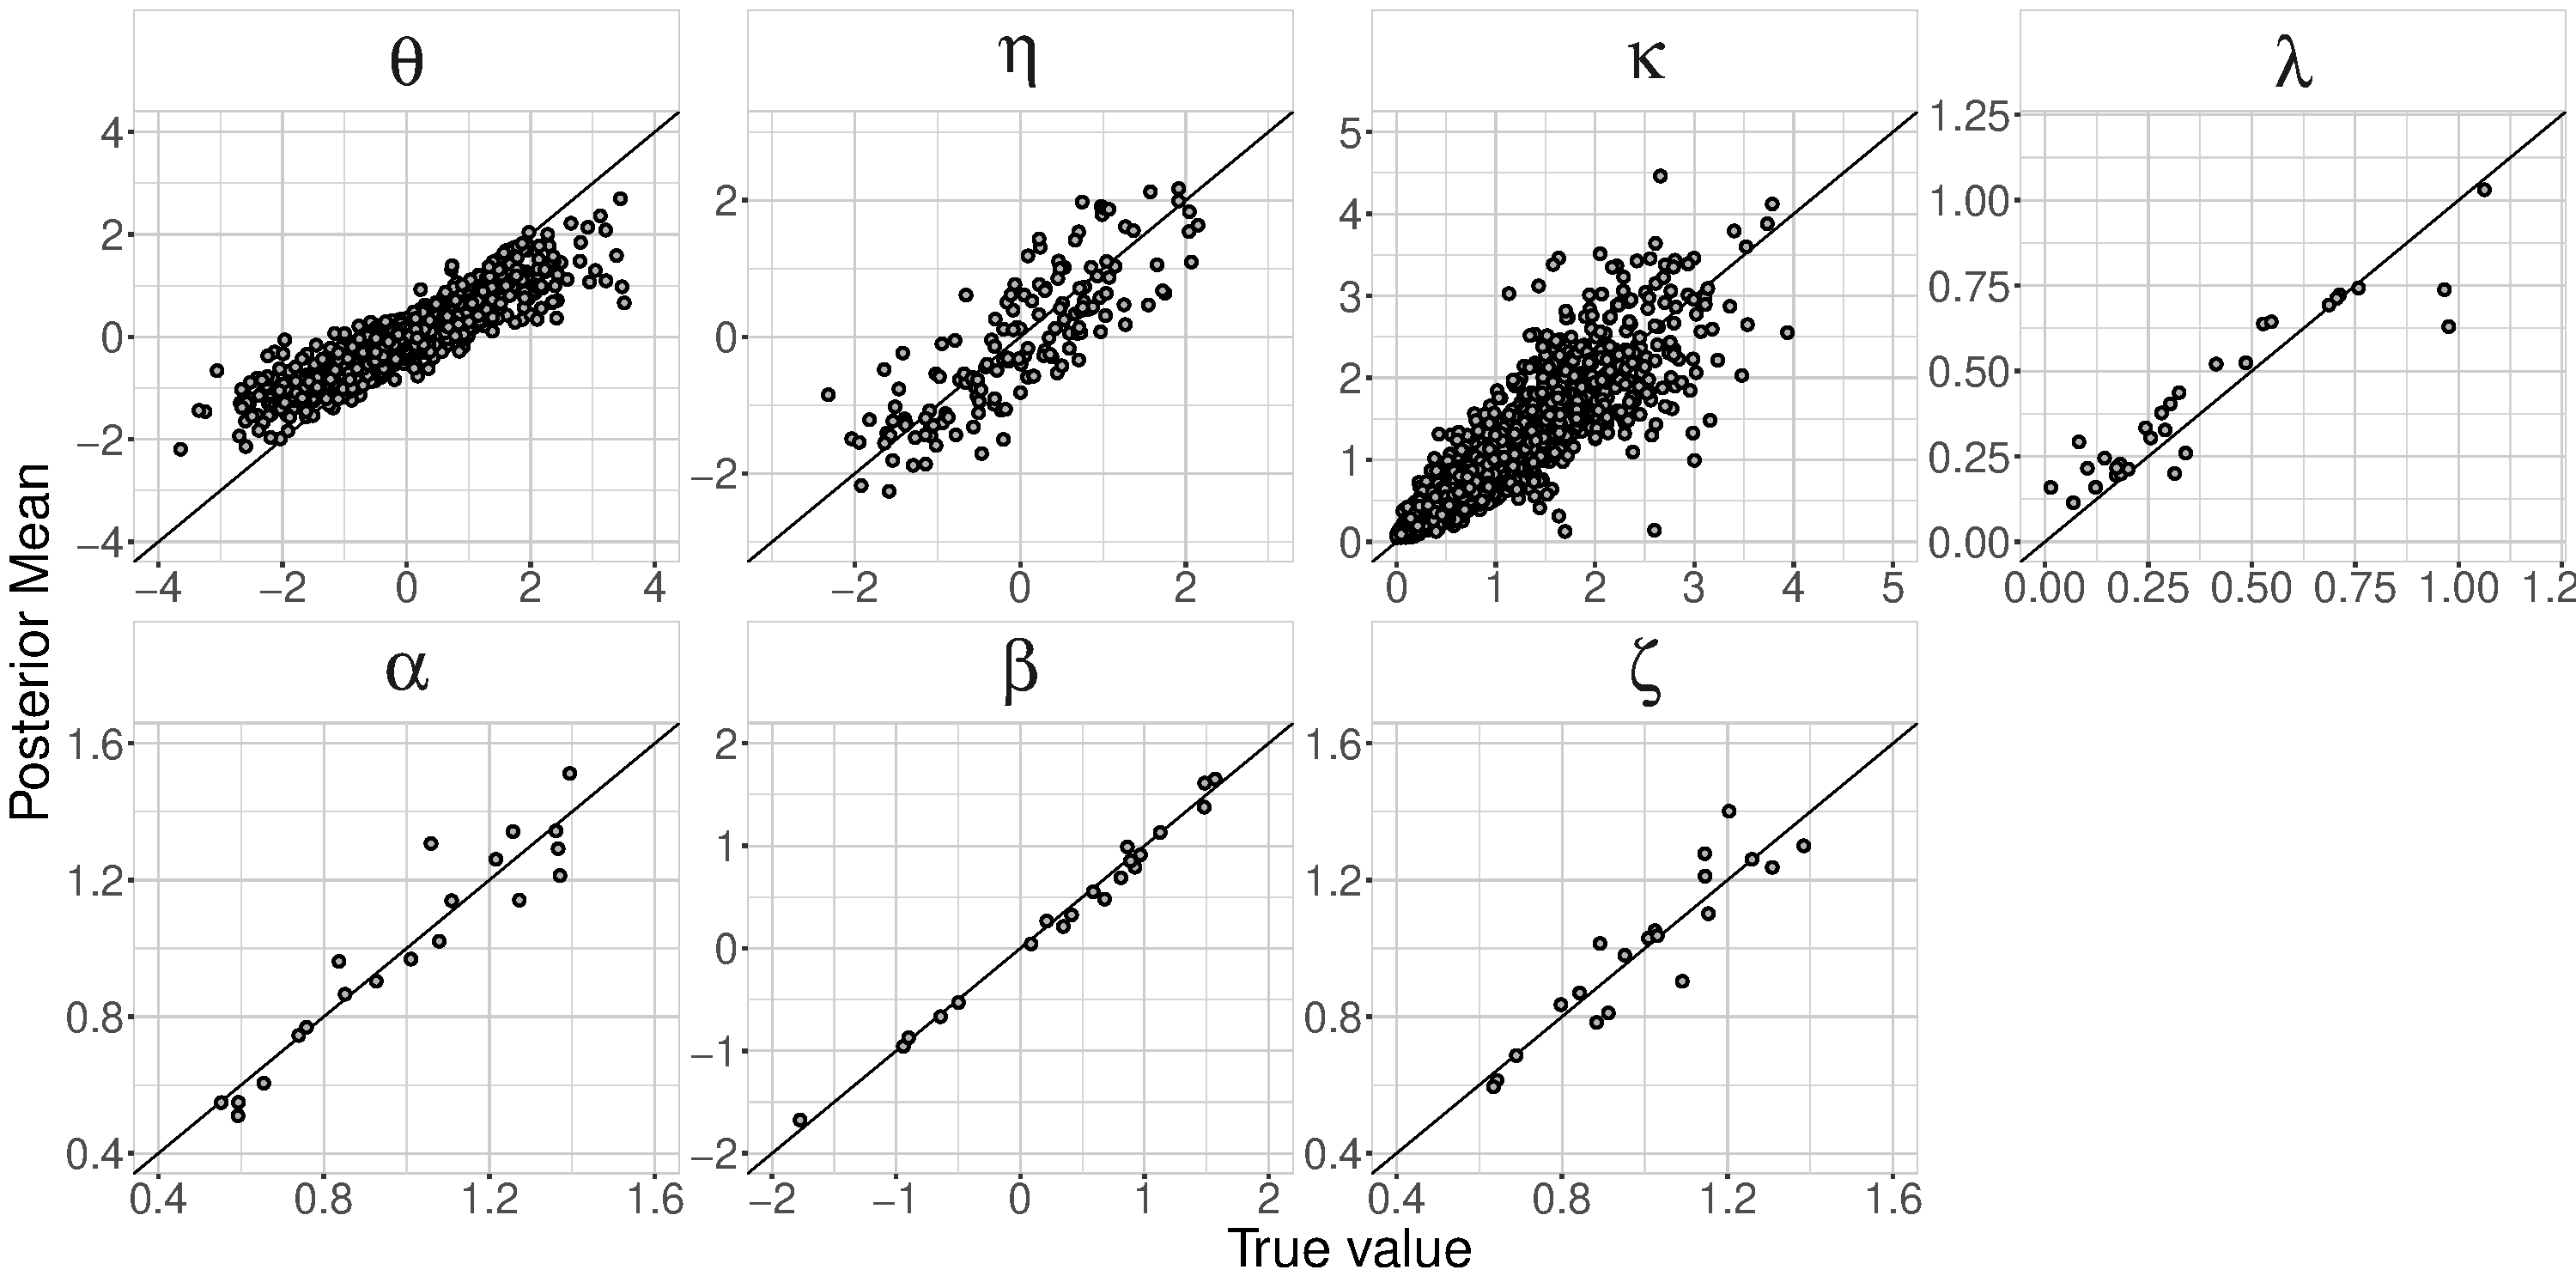
\includegraphics[width= \textwidth]{figures/parameterRecoveryModel2.pdf}
	\caption{True value used for data simulation (x-axis) and posterior mean of that parameter (y-axis), for all parameters of the LTRM. Above each panel is indicated which parameter is shown.}
	\label{fig:parameterRecoveryELTRM}
\end{figure}

All parameters are retrieved adequately. An exception is the item difficulty $\ItemDifficulty$ whose estimates appear more variable as the true item difficulty increases. The spread in posterior means of the item difficulty is similar to that in Figure~6 in \AB{}. The item truths $\ItemTruth$ seem underestimated as their magnitude increases. The hierarchical structure of the extended LTRM likely shrinks the item truths towards the mean. Typically, there is more shrinkage if the values of the parameter are larger, as is the case here. This bias does not appear to influence the other parameter much, as the latent constructs $\FactorScore$ are retrieved accurately. %Also, the posterior means of $\mu_\beta$ are approximately equal to the sample means of $\RaterShift_\Irater$ split by the rater specific covariates. These sample means differ somewhat from the true means since there are 5 observations per mean.

Although it is good to know when the parameters of the extended LTRM can be recovered, it may be more useful to know when the data are not sufficiently informative to apply the extended LTRM. This is likely the case when there are few items and raters. Exact numbers, however, may vary depending on the specific situation at hand. For most purposes, it is straightforward to adjust the number of raters, items, and patients, and then repeat the simulation. As an exercise, we also recovered the parameters for \AB{}'s LTRM. Code for the simulation is available in the online appendix and parameter recovery is shown in Figure~\ref{fig:parameterRecoveryABLTRM}.

\subsection*{Predictive Performance}
Here, we compare the predictive performance of the LTRM to that of the sample mode and, as a more informative comparison, to Random Forest and Boosted Regression Trees (Boosting). Random Forest and Boosting analyses were done using the R packages \code{ranger} and \code{gbm} respectively \cite{ranger2017, gbmPackage}. We used the default settings for the hyperparameters in both R packages.

We simulated two data sets each consisting of 20 raters, 30 items, 50 patients, and thus in total 30,000 observations. The first data set represented a dense design, where all raters scored all patients. The second data set represented a sparse design, where each rater scored 10 patients. Raters were assigned to patients so that the number of obtained scores was about equal for all patients. To simulate a sparse data set, we first simulated a dense data set and subsequently removed a score if the raters that did not rate a patient. This remaining sparse data set consisted of 6,000 observations. Next, both data sets were split into a training set (80\%) and a test set (20\%). The performance of the four methods was evaluated by training the models on the training set and using the trained model to predict the outcomes for a test set. For the LTRM, we used the mean of the posterior predictive distribution as a point-prediction.\footnote{In this particular example, model predictions could also be interpreted as imputing missing values. If these are regarded as missing observations rather than predictions, they should be modeled as unknown discrete parameters of the model \cite<Ch.~8;>{GelmanEtAl2014BDA}. That way, uncertainty about these missing observations is propagated into the parameters. Although we did not sample the missing observations from the joint posterior distribution, the code in the online appendix does show how to do this.} Predictions for Random Forest and Boosting were obtained by taking the majority vote of the trained classification trees. We used the observed mode of all observations for the same rater, item, or patient (i.e., to predict $x_{\Irater\Iitem\Ipatient}$ we used mode$(x_{-\Irater,\Iitem\Ipatient},x_{\Irater,-\Iitem,\Ipatient},x_{\Irater\Iitem,-\Ipatient})$).\footnote{We used the mode rather than the mean because the mean's predictions lie outside of the ordinal scale and thus prediction accuracy cannot be quantified in the same manner as for the other methods.} 

We quantified predictive performance by computing the confusion matrix between held-out responses and predicted values; a contingency table with correct predictions on the diagonal. Prediction accuracy is defined as the number of correct predictions divided by the total number of predictions.

%\DON{Misschien kunnen we deze paragraaf ook gewoon skippen}
%A technical difference between this approach and the previous simulations is that model predictions are effectively treated as missing data. In terms of implementation, a complete data set, where every patient is scored on each item by all raters, can be represented as an array of dimensions $\Trater\times\Titem\times\Tpatient$. However, it is easier to handle an incomplete data set by representing the data as a matrix of $(\Trater\times\Titem\times\Tpatient)$ rows and $4$ columns (i.e., long format).\footnote{For a Stan implementation, the long format is even required as missing values must be handled explicitly, unlike for other software e.g., JAGS.} In this format, the first column indicates the outcome, the second the rater, the third the item, the fourth the patient, and subsequent columns indicate rater and patient covariates.

\begin{table}[!ht]
	\centering
	\caption{Prediction accuracy for the LTRM, Random Forest, Boosting, and the sample mode. The LTRM outperforms all other methods, but Random Forest and Boosting perform remarkably well. Since the data are simulated the choices for the simulation settings are somewhat arbitrary, and different settings could yield a very accurate of very inaccurate predictive performance (e.g., by adjusting item difficulty and rater competence). Therefore, the absolute prediction error cannot be interpreted and only a relative comparison should be made. Since there were 5 possible outcomes, an accuracy of $0.2$ would be chance performance.}
	\begin{tabular}{lrr}
		\toprule
		Method        & Dense & Sparse \\
		\midrule
		LTRM          & 0.52  & 0.46 \\
		Sample Mode   & 0.43  & 0.43 \\
		Random Forest & 0.42  & 0.42 \\
		Boosting      & 0.39  & 0.40 \\
		\bottomrule
	\end{tabular}
\end{table}
Given that the data were generated by the LTRM, it comes as no surprise that it predicts more accurately than the other methods. However, even though data generated from the LTRM is likely a gross simplification of reality, the results show that black-box machine learning methods perform somewhat adequately. This is somewhat surprising because the data at hand are ill-suited for black-box machine learning methods, as these have difficulty capturing the hierarchical structure of the data which contains most of the information \cite<but see>{hajjem2014mixed}. Instead, if a lot of background information about patients and raters is available, this could likely improve their performance. However, machine learning methods do not provide interpretable models, which may be undesirable in practice because it makes it difficult to substantiate decisions. 
 
\section*{Discussion}

In this paper, we extended the Cultural Consensus model developed by \citeA{Anders2015cultural} so as to apply to patients' mental health scores. The original model was suited for data from a single patient and we extended this to multiple patients, latent constructs, and patient and rater specific covariates. The benefit of this approach is that we can obtain estimates for, for example, a patients aggressiveness while accounting for rater bias, item-specific measurement error, and the nature of a patient's previous criminal offense. We have shown in a simulation that the parameters of the extended LTRM can be retrieved accurately.

Although the LTRM provided better predictions than black-box machine learning approaches, this is likely because the data were simulated from the LTRM. It seems more reasonable that an optimal method for prediction would combine results from the LTRM with some machine learning approach. For example, augmenting a Random forest model with features based on psychological theories resulted in a model with better predictions of human decisions than models based on psychological theories or naive machine learning models \cite{plonsky2019predicting, plonsky2017psychological}. However, machine learning approaches, despite their predictive power, result in uninterpretable models which may be undesirable in psychiatric practice where decisions need to be motivated and possibly defended (e.g., when determining whether a treatment is effective or when deciding if a patient should be released).

Ideally, patients are monitored over some time and data from multiple measurement occasions is obtained and analyzed using the extended LTRM. Rather than applying the LTRM repeatedly to data from individual measurement occasions, all observations should be analyzed simultaneously. That way, a patient's progress may be monitored over time and predictions for the future time points could be obtained along with uncertainty estimates. To extend the LTRM to incorporate time-varying components is conceptually straightforward, but the exact properties of the time-varying components should depend on the data at hand. For example, one can imagine that the factor scores of a patient vary over time as described by a dynamic factor model \cite{molenaar1985dynamic, forni2000generalized}. However, when patients are rated only rarely -- say every six months -- then the application of a sophisticated time series model is not feasible. Instead, simply estimating the difference between consecutive time points with an intercept may suffice. For these reasons, we did not explore a time series extension of the LTRM.

\subsection*{Limitations}

In the LTRM, we assumed that the factor structure is known. In practice, however, this need not be the case. Estimating the factor structure from the data is possible, although such an endeavor shifts the focus of the LTRM to model selection rather than assessing the progress of patients. Another more flexible approach is to view the latent true scores of the items as a network and estimate the relations among the items (but see \citeNP{Epskamp2017CarefulWish} for possible drawbacks).

Since the posterior distributions were approximated with variational inference, the obtained posterior distributions may be biased. In general, these biases rarely affect the estimated posterior means, but the posterior variance can be underestimated \cite{blei2017variational}. As a consequence, uncertainty estimates may be too narrow. To alleviate this, it is relatively trivial to modify the Stan code in the appendix to use MCMC instead of variational inference (e.g., in the code in the appendix change \code{vb(model)} to \code{sampling(model)} to use MCMC). However, note that MCMC algorithms for the models discussed run for hours to obtain a reasonable number of posterior samples, whereas variational inference finishes after several minutes.

\subsection*{Recommendations for clinical practice}
To successfully apply the extended LTRM in practice, the data should meet several minimum requirements. %These requirements helps to ensure that, for example, the data are not overly noisy to  the data meets a number of minimum requirements
Although the model accounts for differences between raters, it is best to minimize these differences, for instance through clear scoring instructions. In addition, there should be overlap among (groups of) raters and the patients they score. That is, patients should be scored by multiple raters in such a way that there are no isolated groups of raters and patients, where one group of raters only rates one group of patients and another group of raters rates a different group of patients. A lack of overlap between two groups complicates a comparison between raters and patients between them. A lack of overlap can be avoided by having rater 1 score patients 1 through 5, having rater 2 score patients 3 through 7, etc. Additional information about patients should be added to the model, such as the reason for incarceration. That should help the extended LTRM to distinguish between groups of patients that differ on these covariates. This also holds for the raters; if certain background variables are suspect to causing rater bias then these should be included in the model.

In sum, we extended the Latent Truth Rater model (LTRM) introduced by \citeA{Anders2015cultural} to a model that can be applied to patients' mental health scores in psychiatric detention centers. The model accounts for individual differences between raters, items, and patients. We demonstrated that the extended LTRM can provide more information about the data at hand than the raw means for two fictitious patients. In addition, we have shown that the parameters of the extended LTRM can be adequately retrieved and that the LTRM outperforms the observed mode and several machine learning toolboxes in terms of predictive power. Finally, we have provided recommendations for clinical practitioners who wish to apply the LTRM in practice. Altogether, we hope the extended LTRM improves current practices for analyzing mental health scores in psychiatric detention centers. 


\bibliographystyle{apacite}
\bibliography{references}

\newpage
\appendix
\counterwithin{figure}{section}

\section{Example Analysis}

\begin{figure}[!ht]
	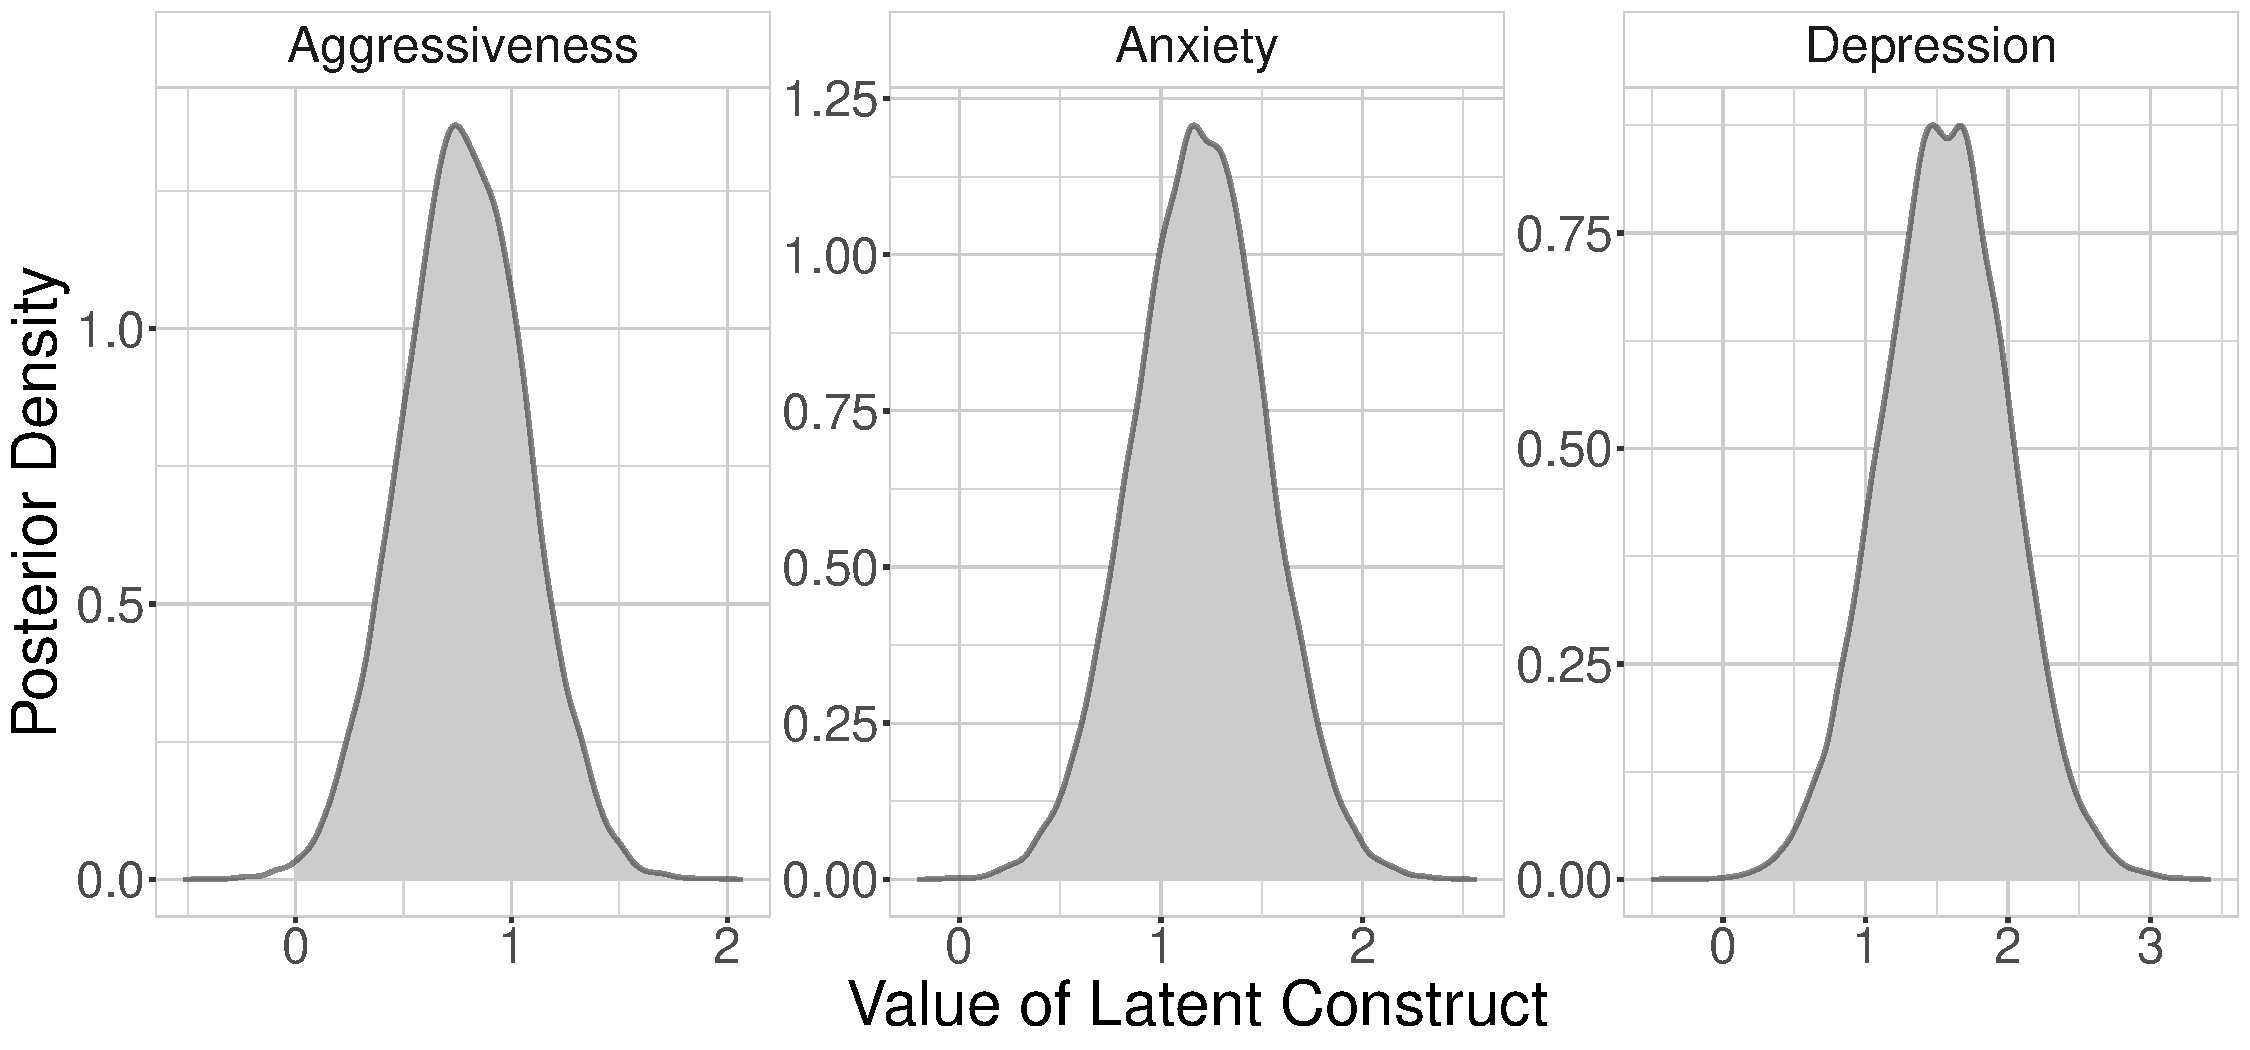
\includegraphics[width=\textwidth]{figures/twoPatientsDiffDensity.pdf}
	\caption{Approximate posterior densities for the differences in latent constructs of two fictitious patients with response pattern. The probability that the difference is larger than 0 is above $0.99$ for all constructs.}
	\label{fig:ExamplePosteriorDiff}
\end{figure}

\begin{figure}[!ht]
\begin{subfigure}{.5\textwidth}
	\centering
	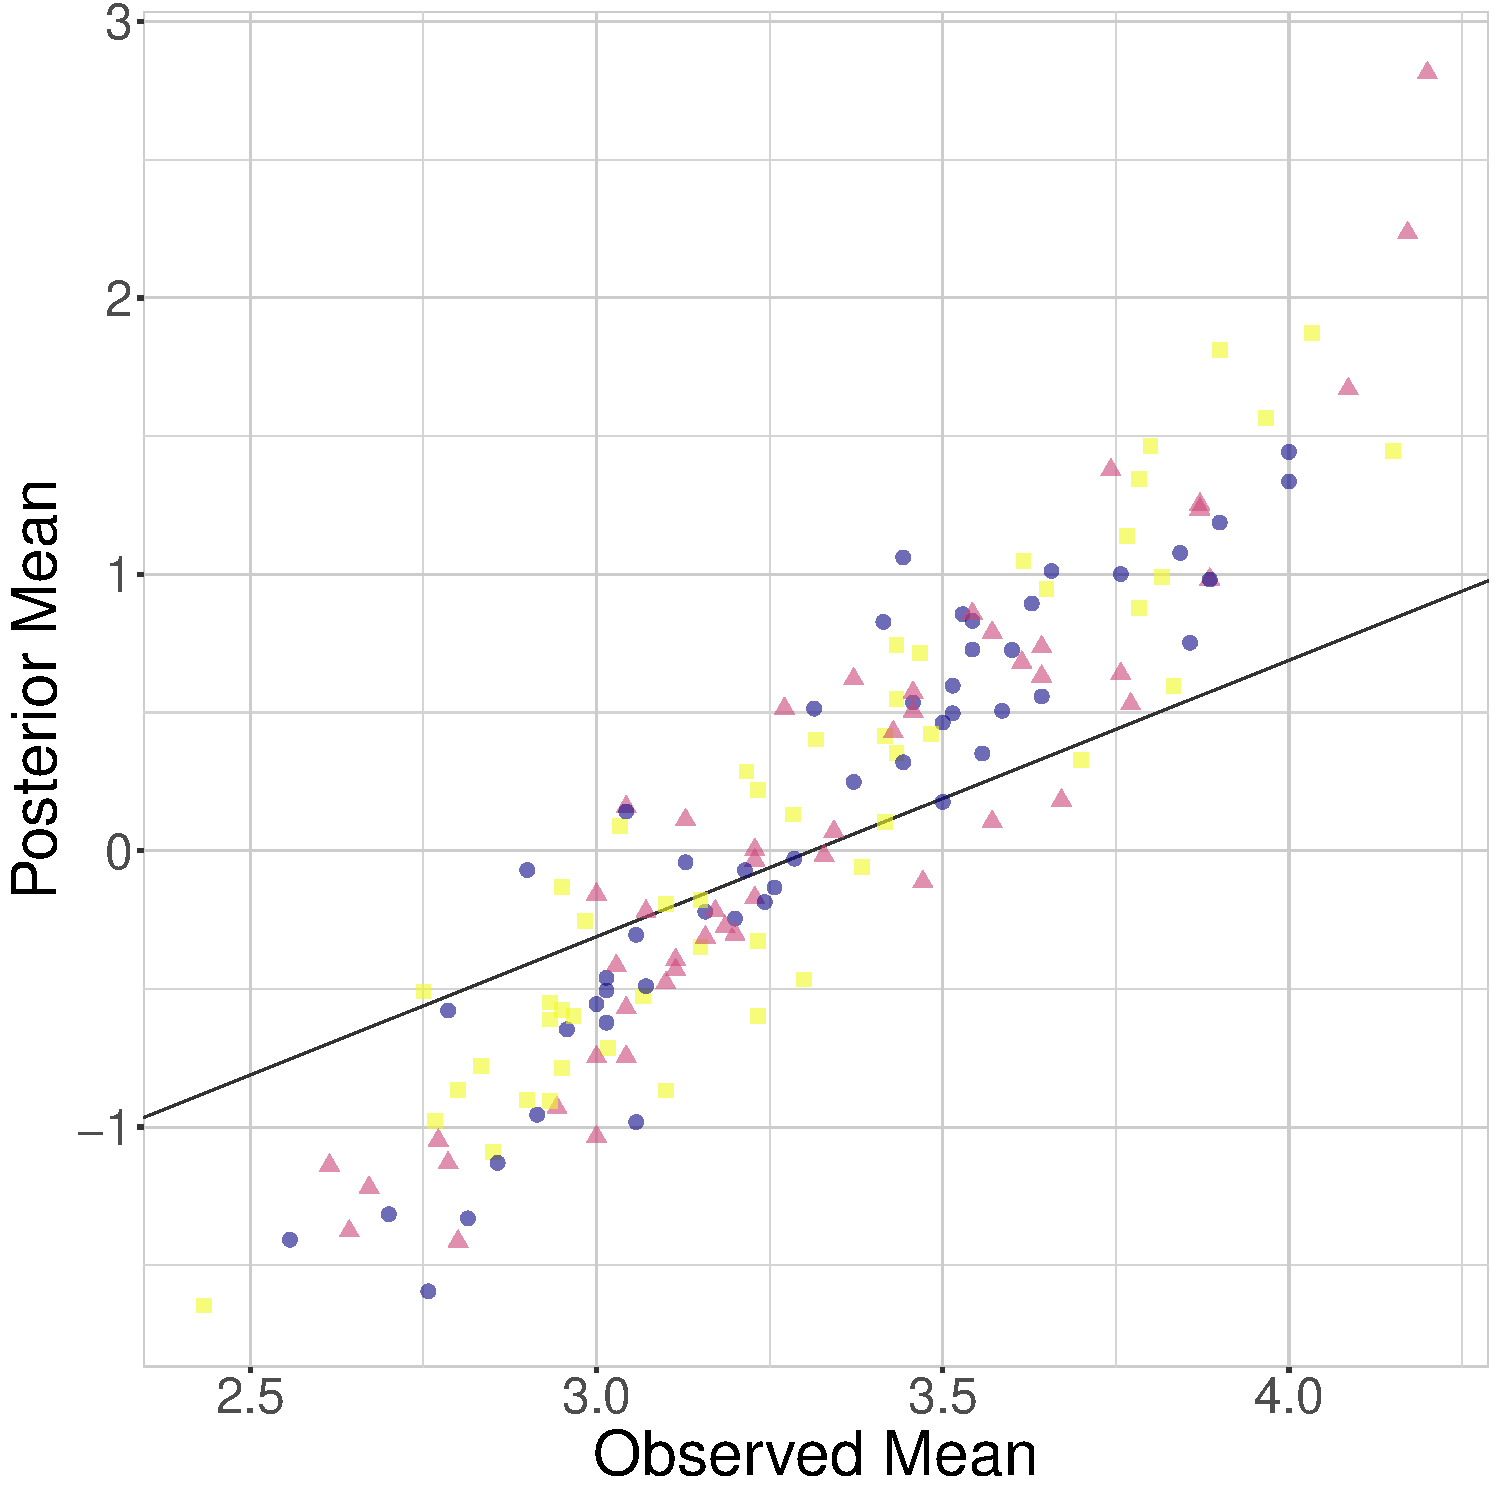
\includegraphics[width=.9\textwidth]{figures/corrObsMeanPostMean.pdf}
\end{subfigure}%
\begin{subfigure}{.5\textwidth}
	\centering
	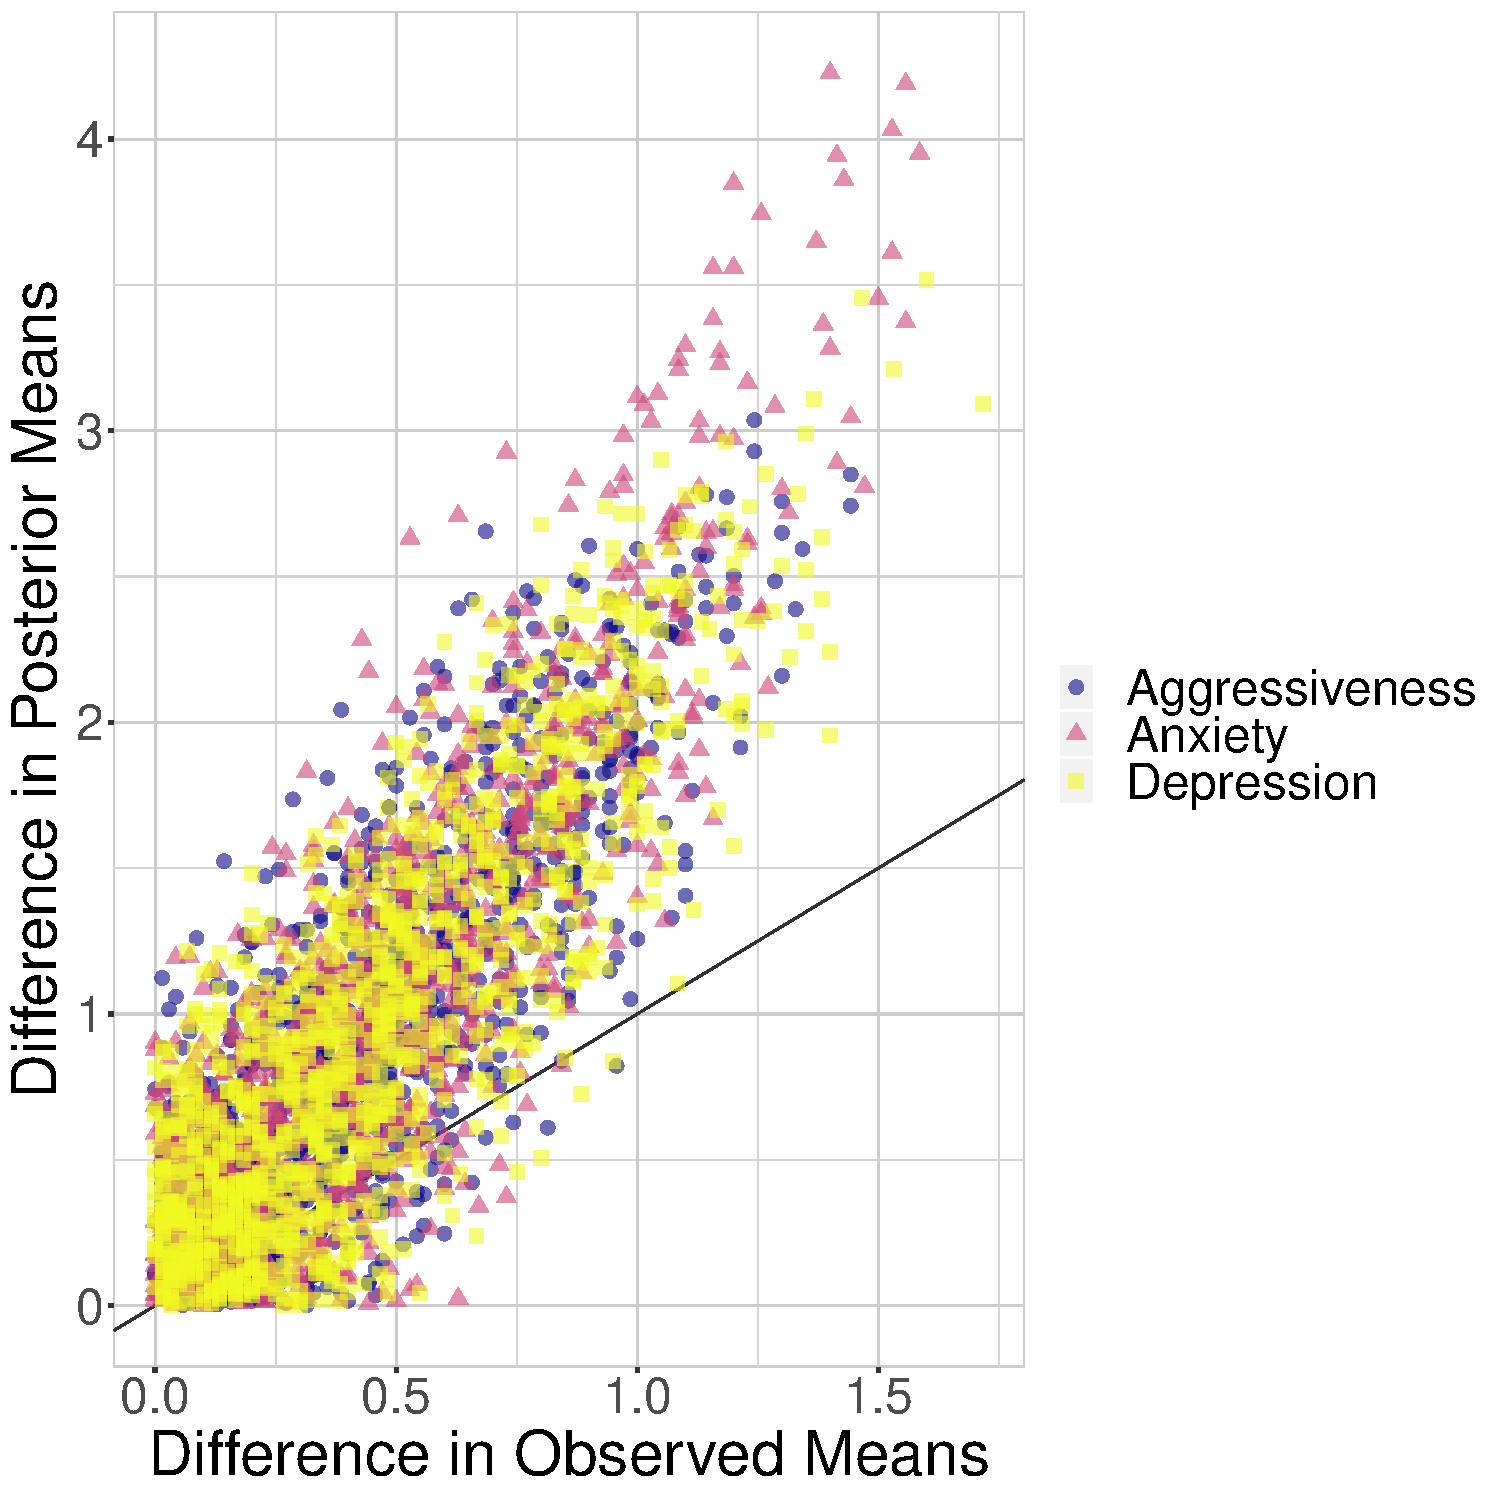
\includegraphics[width=.9\textwidth]{figures/diffCorrObsMeanPostMean.pdf}
\end{subfigure}
\caption{The left panel plots the means of the observed ratings against the posterior means of the latent variables. The right panel shows for each combination of patients $i, j$ the absolute difference in means, $|\hat{x}_i - \hat{x}_j|$, against the absolute difference in posterior means of the latent variables, $|\hat{\eta}_i - \hat{\eta}_j|$. Note that in the left panel, there is a difference in intercept because the responses are on a scale from 1 to 5, whereas the latent variables are assumed to have a mean of 0. The large spread in the right panel demonstrates that the sample mean is an unreliable indicator of the truth underlying the data.}
\label{fig:corrMeanLatentConstruct}
\end{figure}
\newpage

\section{Parameter Recovery}
\begin{figure}[!ht]
	\centering
	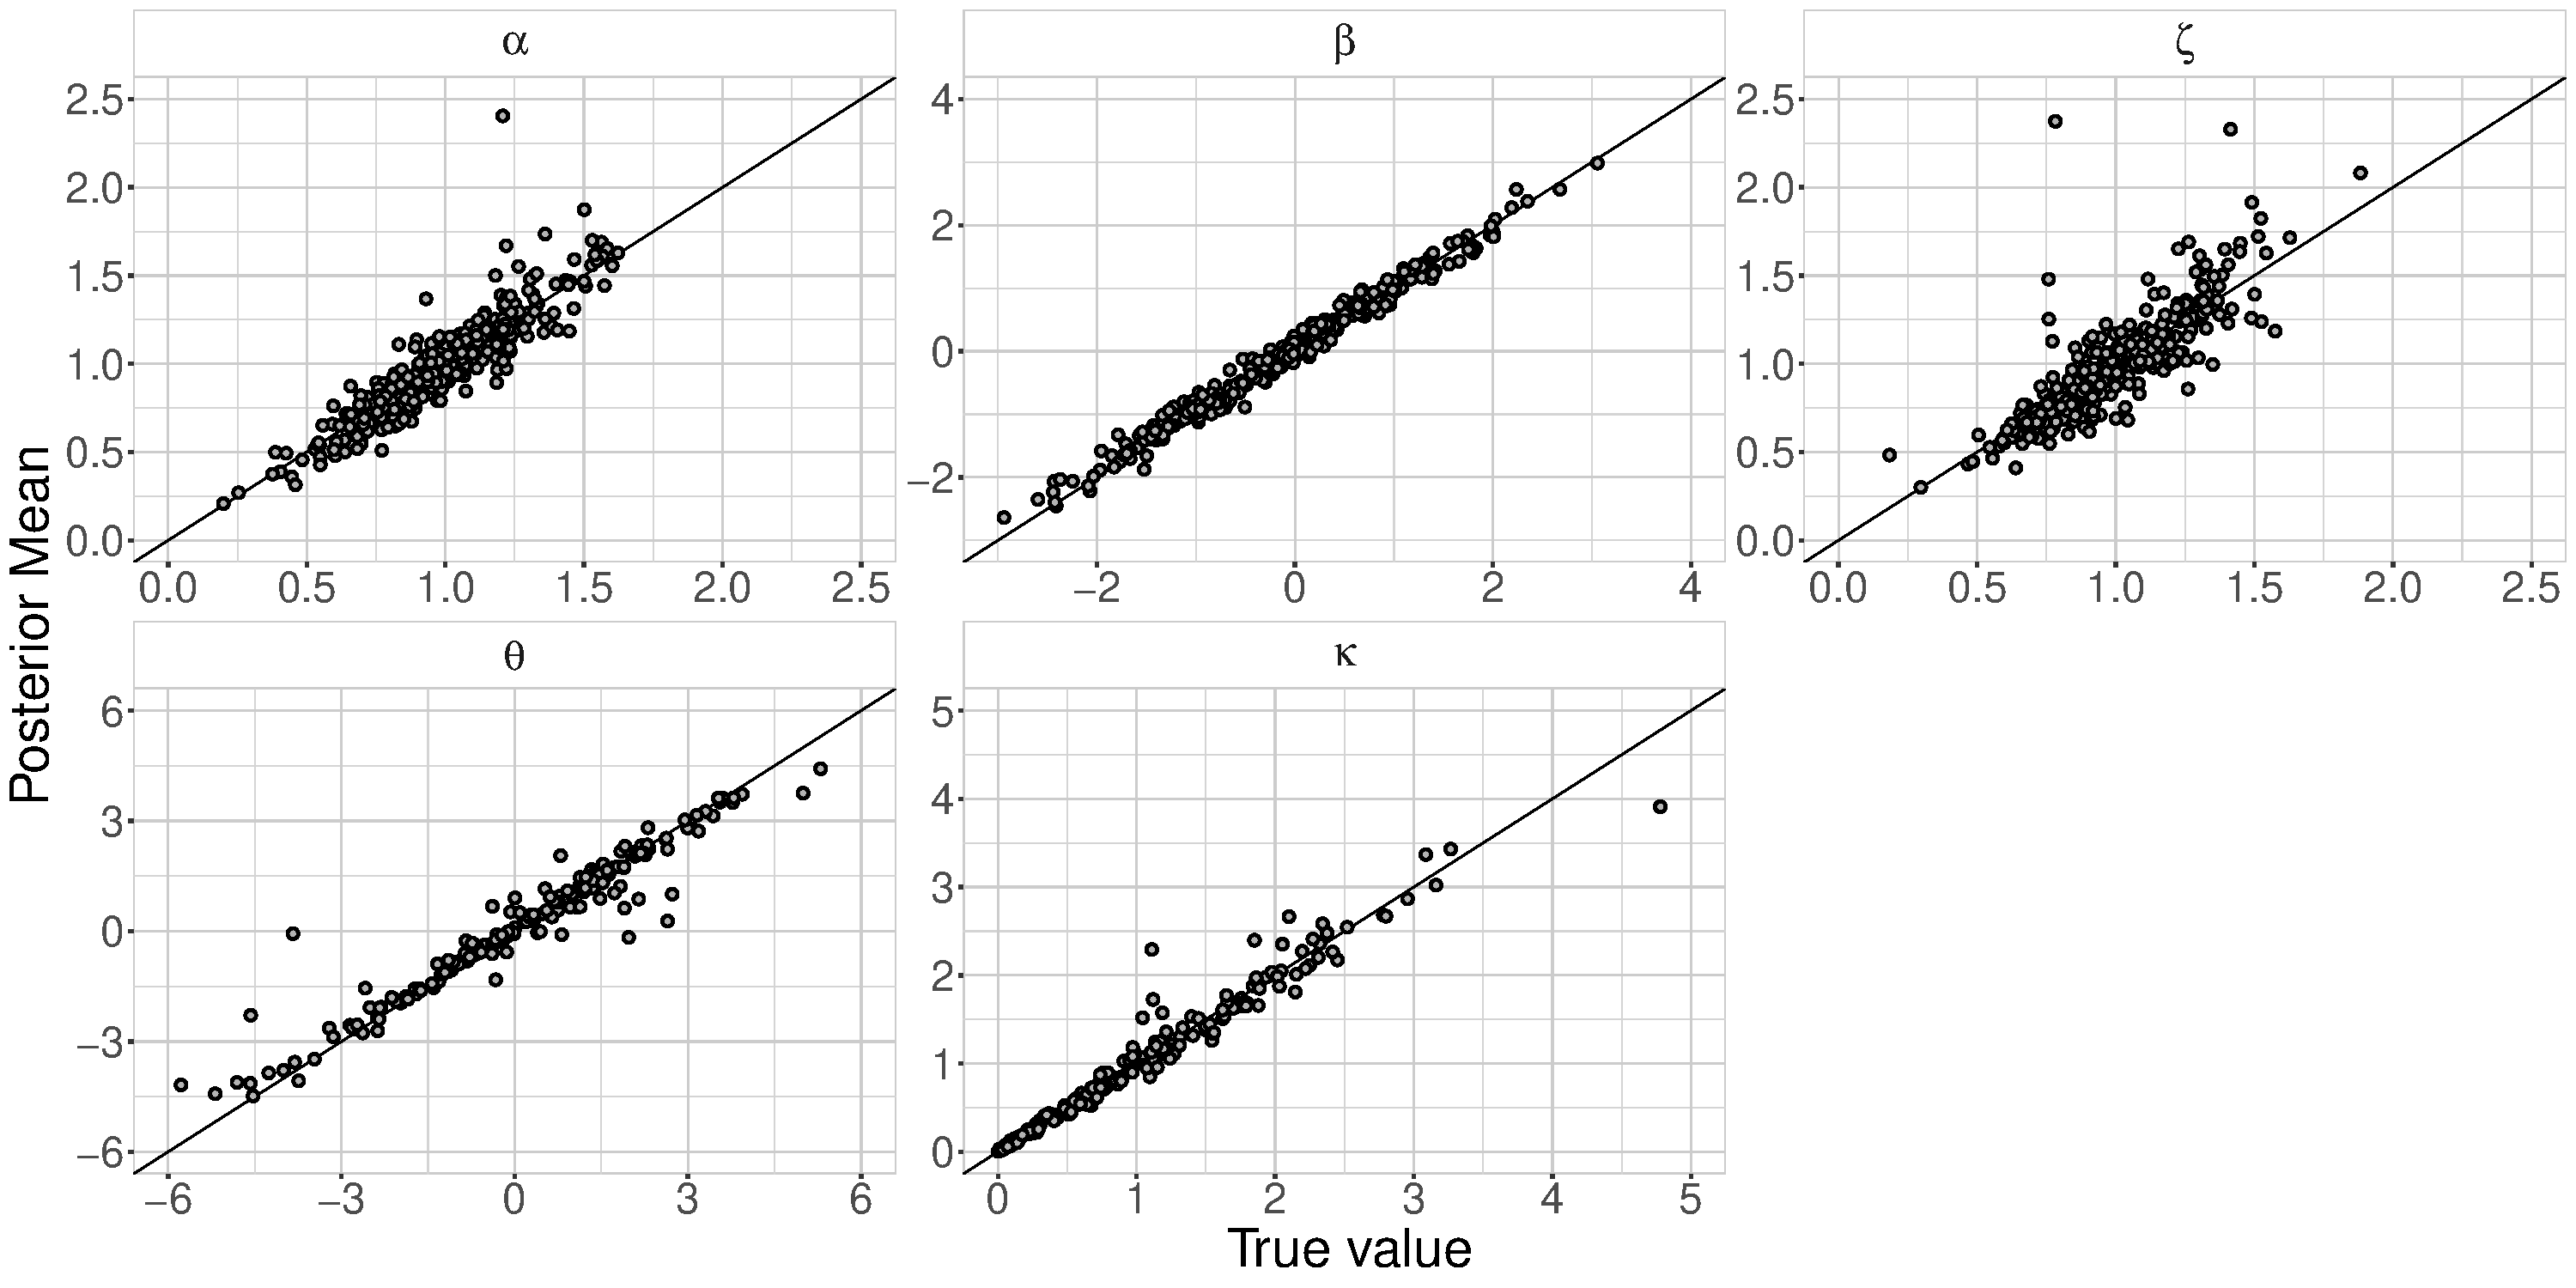
\includegraphics[width= \textwidth]{figures/parameterRecoveryModel1.pdf}
	\caption{Parameter recovery for the Latent Truth Rater model displayed in Figure~\ref{model:LTRM}. The data set consisted of 1 patient, 200 items, and 300 raters. Items had 5 possible outcomes.}
	\label{fig:parameterRecoveryABLTRM}
\end{figure}



%\begin{figure}[!ht]
%	\centering
%	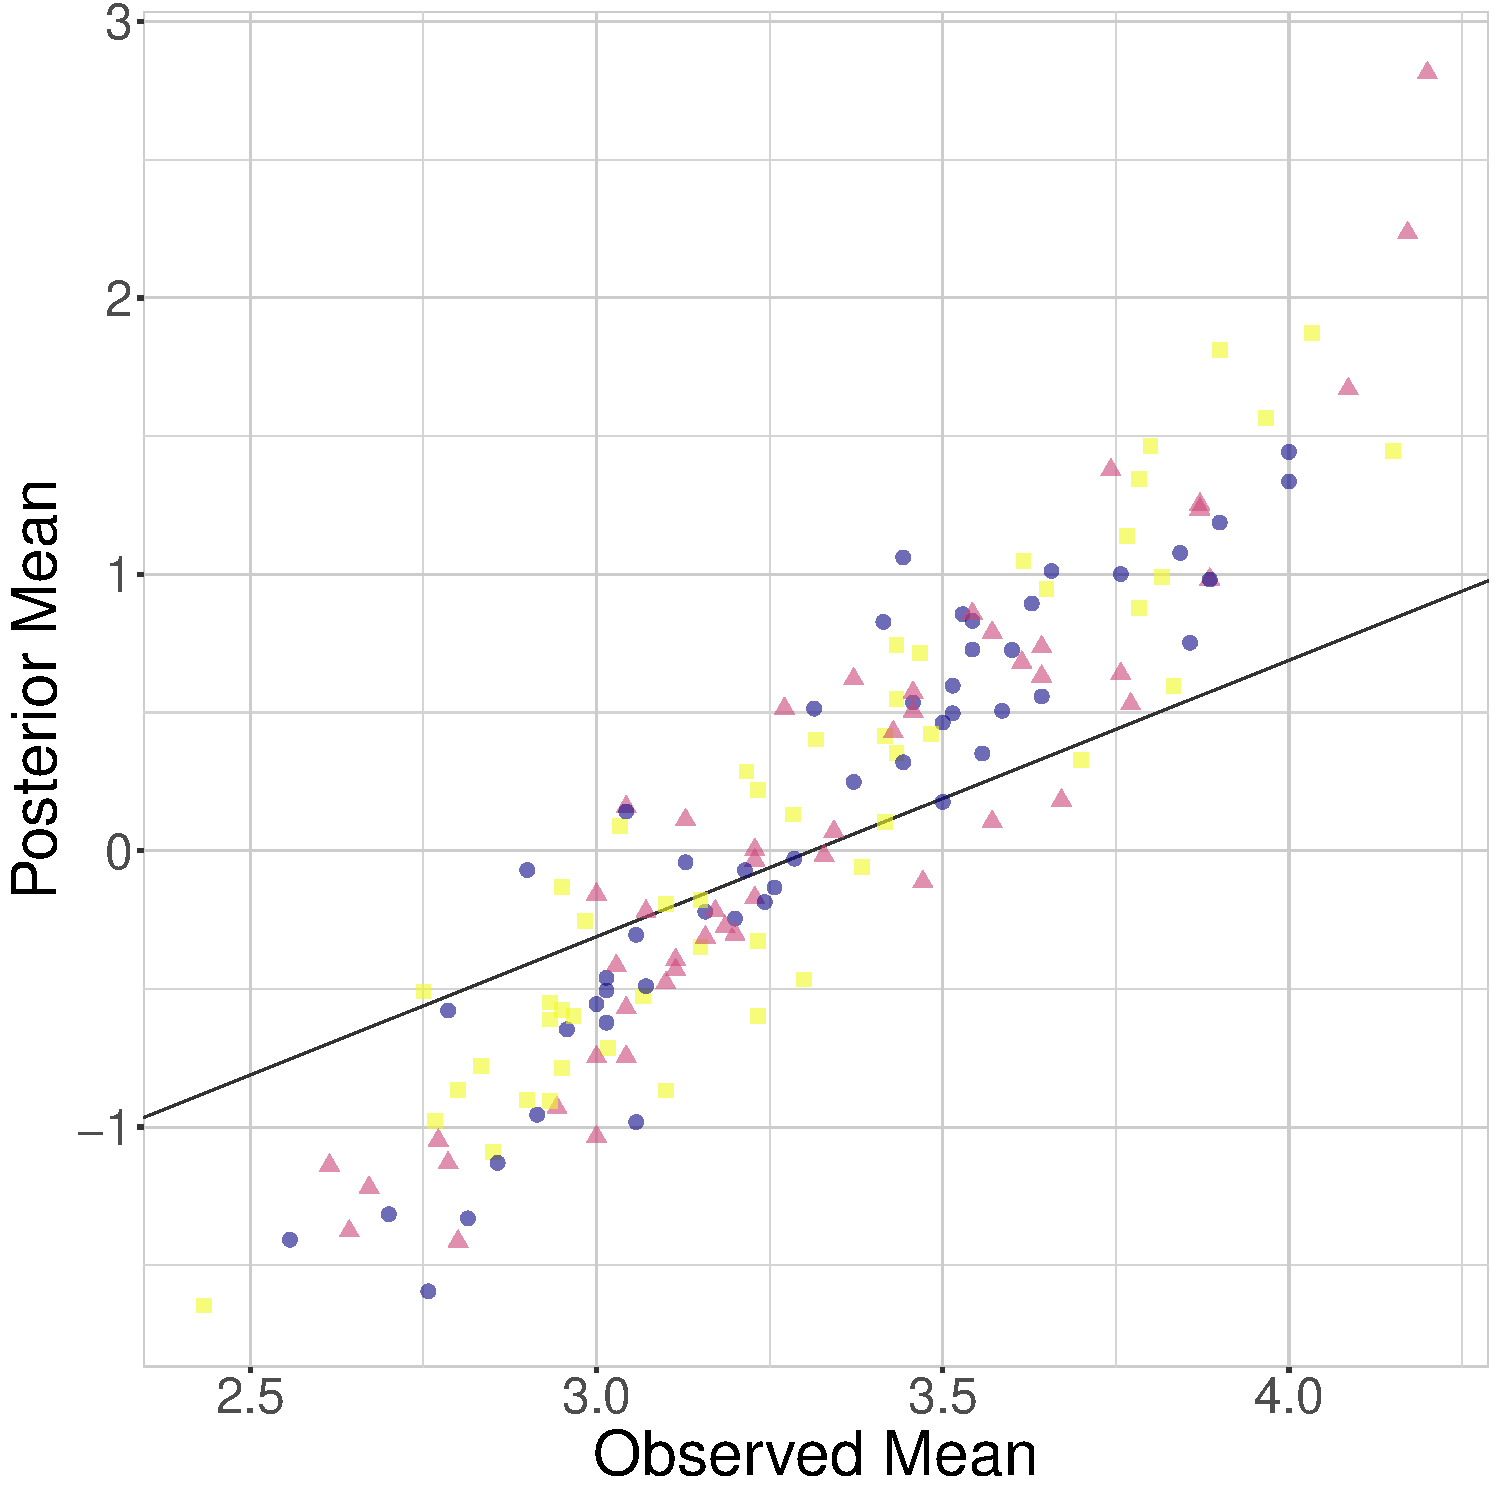
\includegraphics[width= \textwidth]{figures/corrObsMeanPostMean.pdf}
%	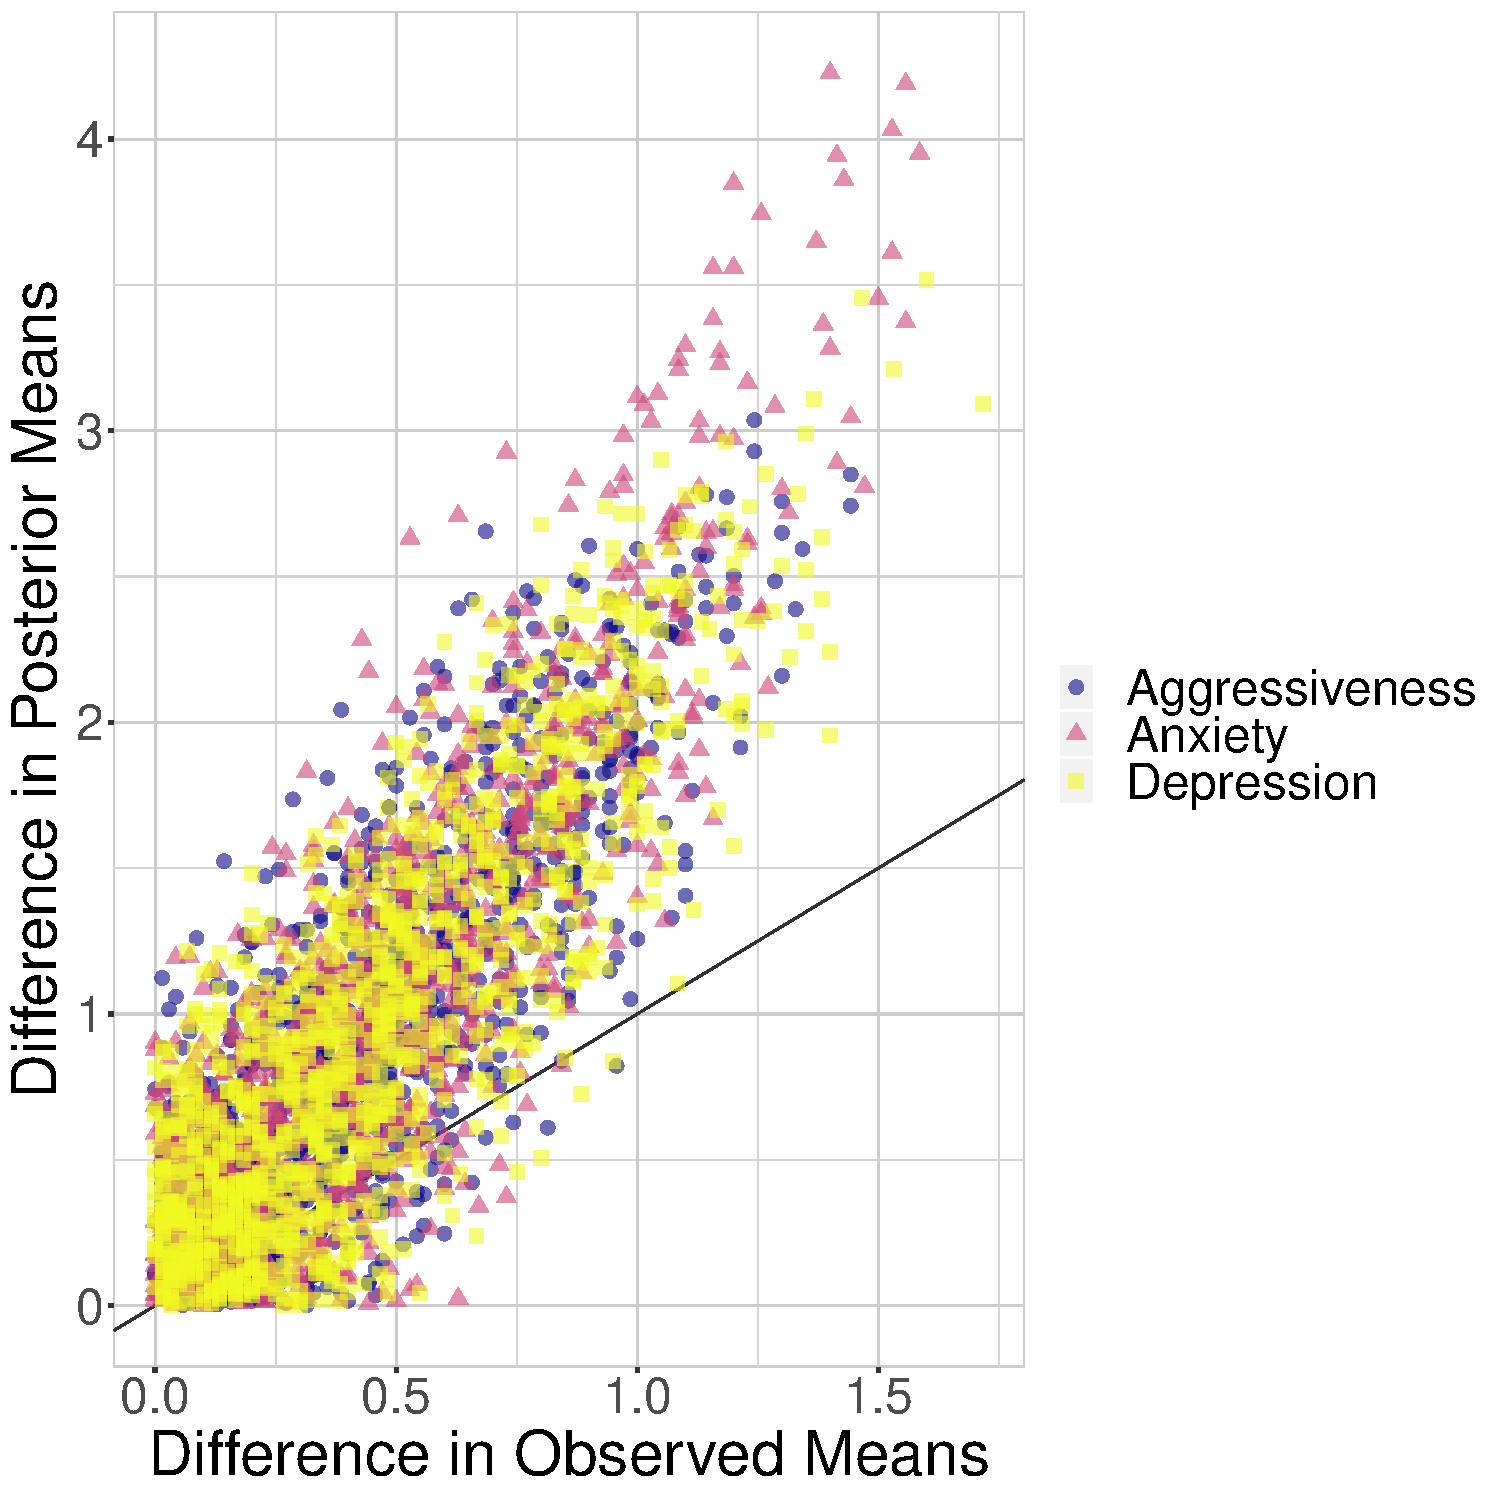
\includegraphics[width= \textwidth]{figures/diffCorrObsMeanPostMean.pdf}
%	\caption{For each patient, a dot on Correlation between the difference scores in posterior mean and the difference in observed mean.}
%	\label{fig:ExampleAnalysisCorrelation}
%\end{figure}



%\begin{figure}[!ht]
%	\centering
%	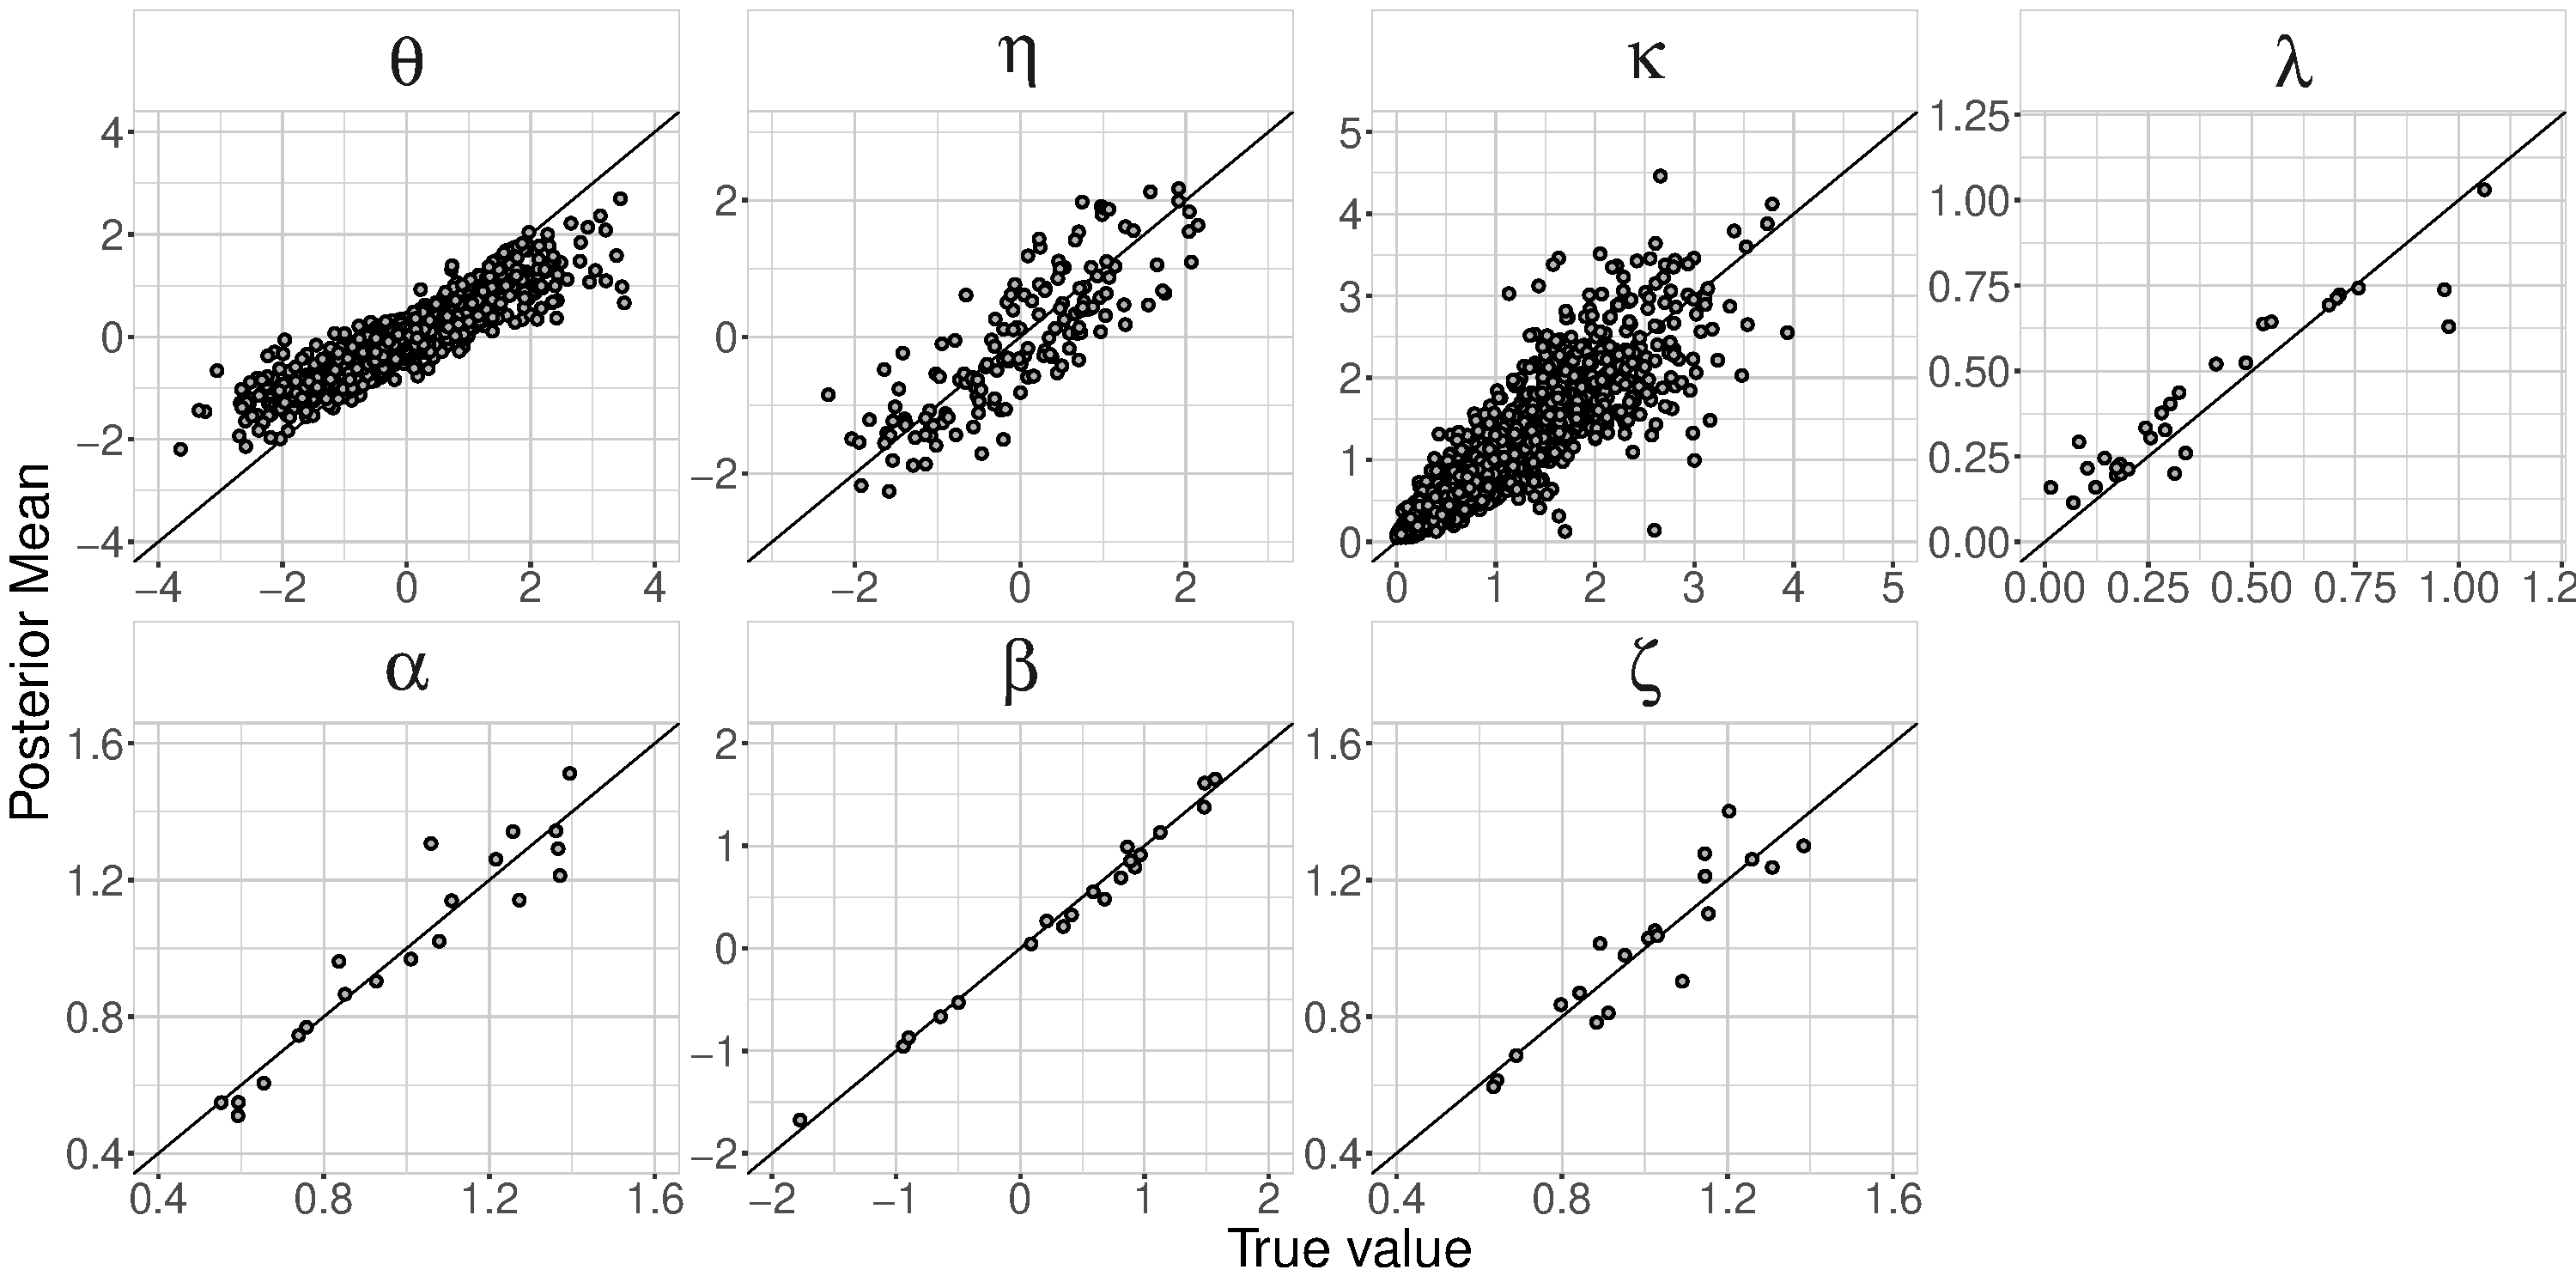
\includegraphics[width= \textwidth]{figures/parameterRecoveryModel2.pdf}
%	\caption{Parameter recovery for the model displayed in Figure~\ref{model:LTRM2}}
%	\label{fig:parameterRecoveryM2}
%\end{figure}

\end{document}

%\subsection*{Progress Monitoring}
%\DON{Naar discussie en voorbeeld over interpretatie uitwerken!}
%
%Ideally, patients are monitored over a period of time and data from multiple measurement occasions is obtained. Next, the LTRM is applied to analyze the data. However, the LTRM should not be applied to data from individual measurement occasions, because an identification restriction of the LTRM is that the mean of each latent construct is zero. Instead, the LTRM can be easily expanded with an intercept that varies across patients, latent constructs, and measurement occasions. As a result, the progress for a single patient on one construct could be visualized as in Figure~\ref{fig:progressMonitoring}.
%
%\begin{figure}[!ht]
%	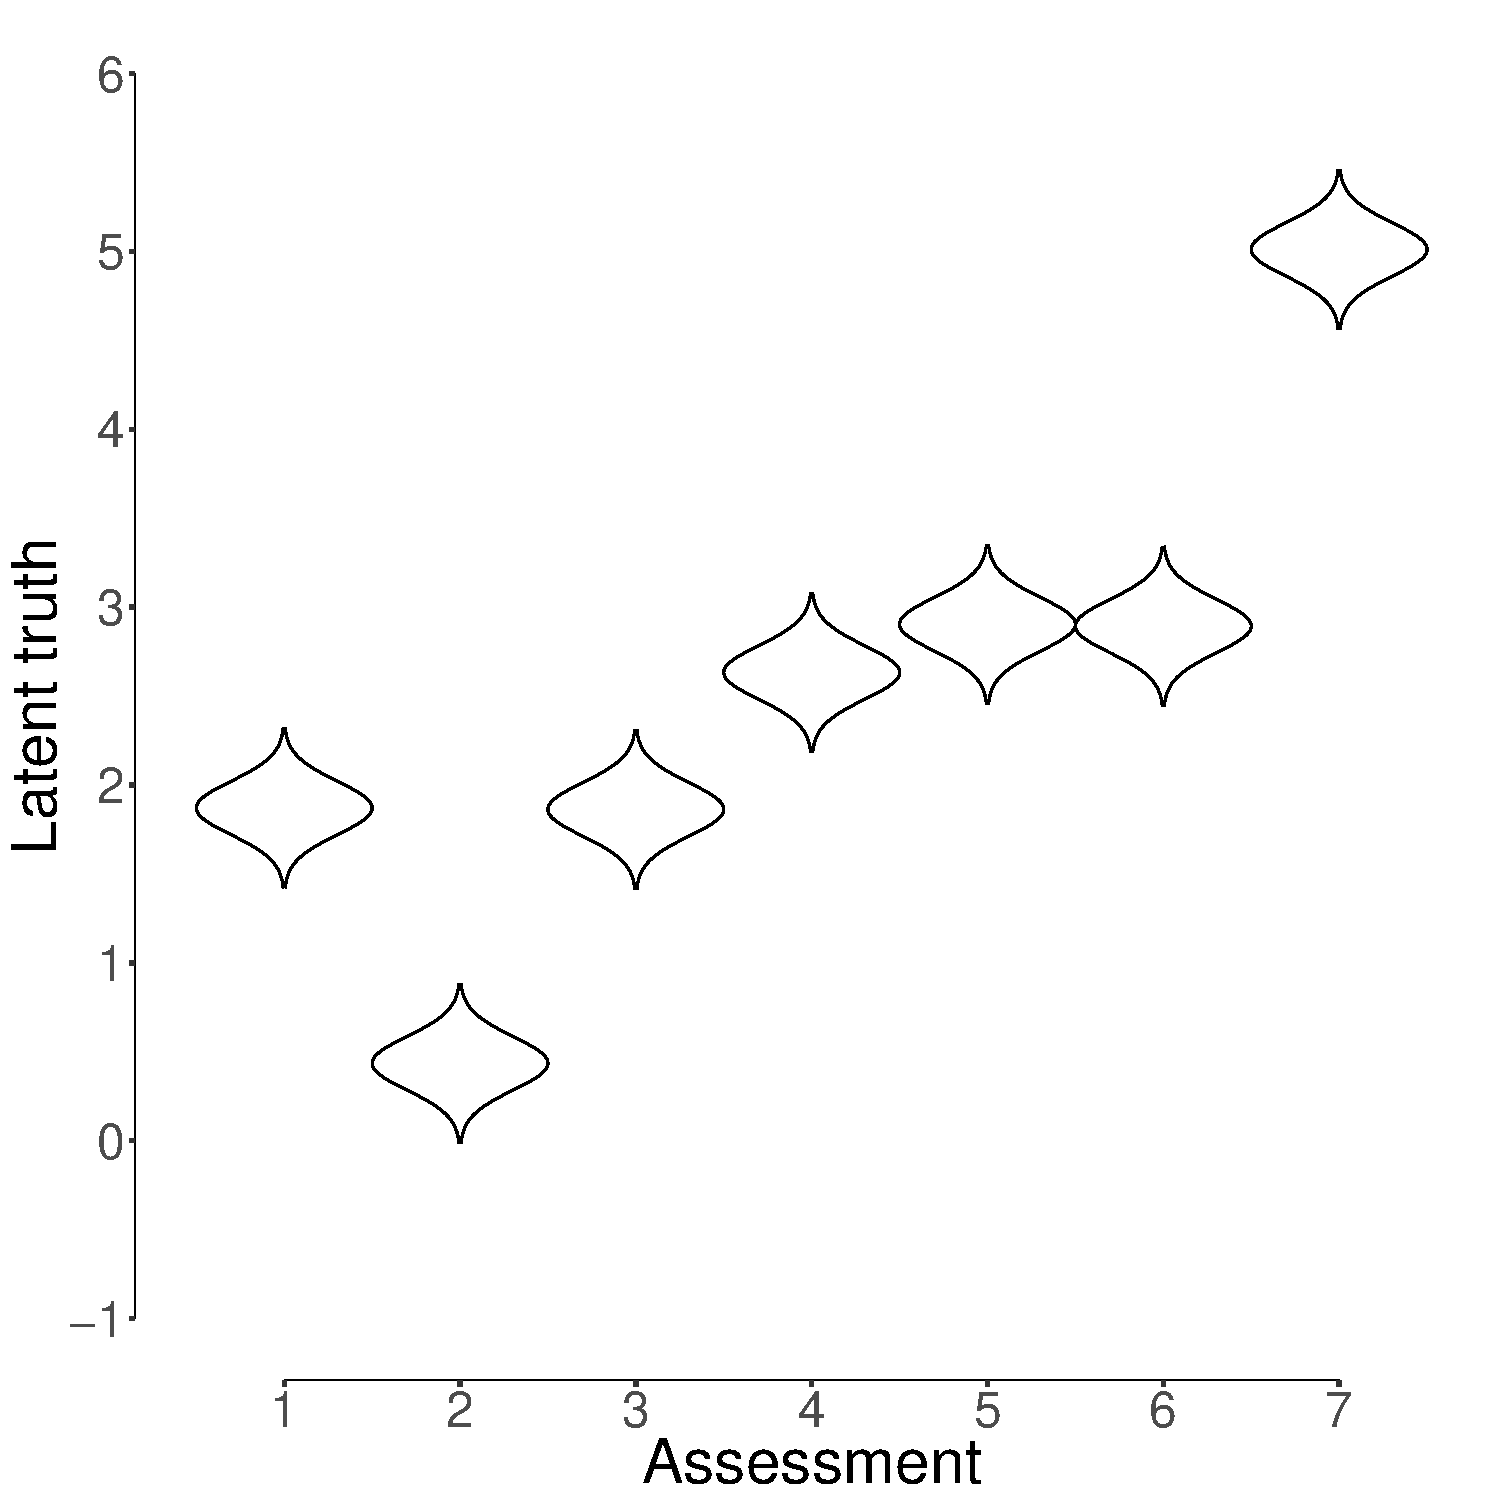
\includegraphics[width=\linewidth]{figures/progressMonitoring.pdf}
%	\caption{Example of how a patient's progress on a single construct could be monitored across measurement occasions.}
%	\label{fig:progressMonitoring}
%\end{figure}

%\newpage
%
%
%personen/ raters zijn gebiased. Kan niet alleen eigenschappen van de gedetineerden halen maar ook die van de raters.
%
%Covariaat voor e.g., hulpverleners versus psychiaters. Meerdere groepen raters (fixed effect).
%
%Hierachisch niveau over patienten.
%
%Covariaat voor groepen gedetineerden (fixed effect misdrijf).
%Ofwel order restrictie voor deze groepen.
%
%Missing values?
%
%Hoe combineren we verschillende schalen van items?
%
%kaart van hoe ontwikkelt zich dit over de tijd (zie figuur in proposal)
%
%TODO: change model in NWO proposal to mimic SDT approach.

%Thus, these models could describe these data. However, currently available CCT models describe data of multiple items and raters, -- but for a single patient.
%The goal of a model appropriate for these data should be to disentangle the patient, rater, and item-specific components in the data. Such a model would benefit decision making because it separates these three different sources of variances and thus decisions can be based on estimates corrected for measurement error. For example, such a model should yield estimates for a patient's aggressiveness, while accounting for rater bias, item-specific measurement error, and a patient's criminal offense. An ideal modeling framework for this is Bayesian hierarchical modeling \cite{ShiffrinEtAl2008}. In particular, Cultural Consensus Theory (CCT), which is designed to pool information from different raters and items, could be seen as a model that accomplishes exactly this -- but for a single patient. \cite{romney1986culture, batchelder1988test, batchelder2012cultural}.
%CCT models describe raters and items using hierarchical structures and thereby accommodates their individual differences. A model based on CCT would allow psychiatric detention centers to assess the effectiveness of their treatments and the mental health of their patients.
%\DON{Iets over goals en benefits!}

%Adding these two concepts to the LTRM model results in the graphical model shown in Figure~\ref{model:LTRM2}.
%\begin{figure}[!ht]
%	\centering
%	\includegraphics[width=.6\textwidth, page=2]{graphicalModels/graphicalModels.pdf}
%	\caption{Graphical model corresponding to the CCT model for multiple patients.}
%	\label{model:LTRM2}
%\end{figure}
%\begin{figure}[!ht]
%\begin{minipage}{0.5\textwidth}
%		\centering
%		\includegraphics[width=1\textwidth, page=2]{graphicalModels/graphicalModels.pdf}
%\end{minipage}\hfill
%\begin{minipage}{0.5\textwidth}
%	{\large
%		\begin{align*}
%		T_{\Iitem\Ipatient} &\sim \dnorm{\lambda_{\Iitem\Ilatent}\eta_{\Ilatent\Ipatient}}{1}\\
%		\eta_{\Ilatent\Ipatient} &\sim \dnorm{0}{1} \\
%		\end{align*}
%	}%
%\end{minipage}
%\caption{Graphical model corresponding to the CCT model for multiple patients.}
%\label{model:LTRM2}
%\end{figure}
%A third extension is to add background information about raters and patients to the model. This would facilitate the model to capture that, for instance, child molesters are less aggressive than murderers. Such patient and raters characteristics could be perceived as covariates and their influence could be captured through a regression on the latent constructs. For instance, the crime of a patient can be regressed on each latent variable, allowing the model to capture that child molesters and murderers differ in aggression, but not in say ... \DONa{ik heb eigenlijk geen idee wat ze allemaal meten}. Rater characteristics could be regressed on the shift of the raters, $\RaterScale_\Irater$. For example, this could capture that some staff members may provide more lenient ratings. Adding these three components to the model results in the graphical model shown in Figure~\ref{model:LTRM3}.
